% Created 2022-11-03 Thu 15:46
% Intended LaTeX compiler: pdflatex
\documentclass[11pt]{article}
\usepackage[utf8]{inputenc}
\usepackage[T1]{fontenc}
\usepackage{graphicx}
\usepackage{longtable}
\usepackage{wrapfig}
\usepackage{rotating}
\usepackage[normalem]{ulem}
\usepackage{amsmath}
\usepackage{amssymb}
\usepackage{capt-of}
\usepackage{hyperref}
\graphicspath{{../../books/}}
% wrong resolution of image
% https://tex.stackexchange.com/questions/21627/image-from-includegraphics-showing-in-wrong-image-size?rq=1

%%%%%%%%%%%%%%%%%%%%%%%%%%%%%%%%%%%%%%
%% TIPS                                 %%
%%%%%%%%%%%%%%%%%%%%%%%%%%%%%%%%%%%%%%
% \substack{a\\b} for multiple lines text
% \usepackage{expl3}
% \expandafter\def\csname ver@l3regex.sty\endcsname{}
% \usepackage{pkgloader}
\usepackage[utf8]{inputenc}

% nfss error
% \usepackage[B1,T1]{fontenc}
\usepackage{fontspec}

% \usepackage[Emoticons]{ucharclasses}
\newfontfamily\DejaSans{DejaVu Sans}
% \setDefaultTransitions{\DejaSans}{}

% pdfplots will load xolor automatically without option
\usepackage[dvipsnames]{xcolor}

%                                                             ┳┳┓   ┓
%                                                             ┃┃┃┏┓╋┣┓
%                                                             ┛ ┗┗┻┗┛┗
% \usepackage{amsmath} mathtools loads the amsmath
\usepackage{amsmath}
\usepackage{mathtools}

\usepackage{amsthm}
\usepackage{amsbsy}

%\usepackage{commath}

\usepackage{amssymb}

\usepackage{mathrsfs}
%\usepackage{mathabx}
\usepackage{stmaryrd}
\usepackage{empheq}

\usepackage{scalerel}
\usepackage{stackengine}
\usepackage{stackrel}



\usepackage{nicematrix}
\usepackage{tensor}
\usepackage{blkarray}
\usepackage{siunitx}
\usepackage[f]{esvect}

% centering \not on a letter
\usepackage{slashed}
\usepackage[makeroom]{cancel}

%\usepackage{merriweather}
\usepackage{unicode-math}
\setmainfont{TeX Gyre Pagella}
% \setmathfont{STIX}
%\setmathfont{texgyrepagella-math.otf}
%\setmathfont{Libertinus Math}
\setmathfont{Latin Modern Math}

 % \setmathfont[range={\smwhtdiamond,\enclosediamond,\varlrtriangle}]{Latin Modern Math}
\setmathfont[range={\rightrightarrows,\twoheadrightarrow,\leftrightsquigarrow,\triangledown,\vartriangle,\precneq,\succneq,\prec,\succ,\preceq,\succeq,\tieconcat}]{XITS Math}
 \setmathfont[range={\int,\setminus}]{Libertinus Math}
 % \setmathfont[range={\mathalpha}]{TeX Gyre Pagella Math}
%\setmathfont[range={\mitA,\mitB,\mitC,\mitD,\mitE,\mitF,\mitG,\mitH,\mitI,\mitJ,\mitK,\mitL,\mitM,\mitN,\mitO,\mitP,\mitQ,\mitR,\mitS,\mitT,\mitU,\mitV,\mitW,\mitX,\mitY,\mitZ,\mita,\mitb,\mitc,\mitd,\mite,\mitf,\mitg,\miti,\mitj,\mitk,\mitl,\mitm,\mitn,\mito,\mitp,\mitq,\mitr,\mits,\mitt,\mitu,\mitv,\mitw,\mitx,\mity,\mitz}]{TeX Gyre Pagella Math}
% unicode is not good at this!
%\let\nmodels\nvDash

 \usepackage{wasysym}

 % for wide hat
 \DeclareSymbolFont{yhlargesymbols}{OMX}{yhex}{m}{n} \DeclareMathAccent{\what}{\mathord}{yhlargesymbols}{"62}

%                                                               ┏┳┓•┓
%                                                                ┃ ┓┃┏┓
%                                                                ┻ ┗┛┗┗

\usepackage{pgfplots}
\pgfplotsset{compat=1.18}
\usepackage{tikz}
\usepackage{tikz-cd}
\tikzcdset{scale cd/.style={every label/.append style={scale=#1},
    cells={nodes={scale=#1}}}}
% TODO: discard qtree and use forest
% \usepackage{tikz-qtree}
\usepackage{forest}

\usetikzlibrary{arrows,positioning,calc,fadings,decorations,matrix,decorations,shapes.misc}
%setting from geogebra
\definecolor{ccqqqq}{rgb}{0.8,0,0}

%                                                          ┳┳┓•    ┓┓
%                                                          ┃┃┃┓┏┏┏┓┃┃┏┓┏┓┏┓┏┓┓┏┏
%                                                          ┛ ┗┗┛┗┗ ┗┗┗┻┛┗┗ ┗┛┗┻┛
%\usepackage{twemojis}
\usepackage[most]{tcolorbox}
\usepackage{threeparttable}
\usepackage{tabularx}

\usepackage{enumitem}
\usepackage[indLines=false]{algpseudocodex}
\usepackage[]{algorithm2e}
% \SetKwComment{Comment}{/* }{ */}
% \algrenewcommand\algorithmicrequire{\textbf{Input:}}
% \algrenewcommand\algorithmicensure{\textbf{Output:}}
% wrong with preview
\usepackage{subcaption}
\usepackage{caption}
% {\aunclfamily\Huge}
\usepackage{auncial}

\usepackage{float}

\usepackage{fancyhdr}

\usepackage{ifthen}
\usepackage{xargs}

\definecolor{mintedbg}{rgb}{0.99,0.99,0.99}
\usepackage[cachedir=\detokenize{~/miscellaneous/trash}]{minted}
\setminted{breaklines,
  mathescape,
  bgcolor=mintedbg,
  fontsize=\footnotesize,
  frame=single,
  linenos}
\usemintedstyle{xcode}
\usepackage{tcolorbox}
\usepackage{etoolbox}



\usepackage{imakeidx}
\usepackage{hyperref}
\usepackage{soul}
\usepackage{framed}

% don't use this for preview
%\usepackage[margin=1.5in]{geometry}
% \usepackage{geometry}
% \geometry{legalpaper, landscape, margin=1in}
\usepackage[font=itshape]{quoting}

%\LoadPackagesNow
%\usepackage[xetex]{preview}
%%%%%%%%%%%%%%%%%%%%%%%%%%%%%%%%%%%%%%%
%% USEPACKAGES end                       %%
%%%%%%%%%%%%%%%%%%%%%%%%%%%%%%%%%%%%%%%

%%%%%%%%%%%%%%%%%%%%%%%%%%%%%%%%%%%%%%%
%% Algorithm environment
%%%%%%%%%%%%%%%%%%%%%%%%%%%%%%%%%%%%%%%
\SetKwIF{Recv}{}{}{upon receiving}{do}{}{}{}
\SetKwBlock{Init}{initially do}{}
\SetKwProg{Function}{Function}{:}{}

% https://github.com/chrmatt/algpseudocodex/issues/3
\algnewcommand\algorithmicswitch{\textbf{switch}}%
\algnewcommand\algorithmiccase{\textbf{case}}
\algnewcommand\algorithmicof{\textbf{of}}
\algnewcommand\algorithmicotherwise{\texttt{otherwise} $\Rightarrow$}

\makeatletter
\algdef{SE}[SWITCH]{Switch}{EndSwitch}[1]{\algpx@startIndent\algpx@startCodeCommand\algorithmicswitch\ #1\ \algorithmicdo}{\algpx@endIndent\algpx@startCodeCommand\algorithmicend\ \algorithmicswitch}%
\algdef{SE}[CASE]{Case}{EndCase}[1]{\algpx@startIndent\algpx@startCodeCommand\algorithmiccase\ #1}{\algpx@endIndent\algpx@startCodeCommand\algorithmicend\ \algorithmiccase}%
\algdef{SE}[CASEOF]{CaseOf}{EndCaseOf}[1]{\algpx@startIndent\algpx@startCodeCommand\algorithmiccase\ #1 \algorithmicof}{\algpx@endIndent\algpx@startCodeCommand\algorithmicend\ \algorithmiccase}
\algdef{SE}[OTHERWISE]{Otherwise}{EndOtherwise}[0]{\algpx@startIndent\algpx@startCodeCommand\algorithmicotherwise}{\algpx@endIndent\algpx@startCodeCommand\algorithmicend\ \algorithmicotherwise}
\ifbool{algpx@noEnd}{%
  \algtext*{EndSwitch}%
  \algtext*{EndCase}%
  \algtext*{EndCaseOf}
  \algtext*{EndOtherwise}
  %
  % end indent line after (not before), to get correct y position for multiline text in last command
  \apptocmd{\EndSwitch}{\algpx@endIndent}{}{}%
  \apptocmd{\EndCase}{\algpx@endIndent}{}{}%
  \apptocmd{\EndCaseOf}{\algpx@endIndent}{}{}
  \apptocmd{\EndOtherwise}{\algpx@endIndent}{}{}
}{}%

\pretocmd{\Switch}{\algpx@endCodeCommand}{}{}
\pretocmd{\Case}{\algpx@endCodeCommand}{}{}
\pretocmd{\CaseOf}{\algpx@endCodeCommand}{}{}
\pretocmd{\Otherwise}{\algpx@endCodeCommand}{}{}

% for end commands that may not be printed, tell endCodeCommand whether we are using noEnd
\ifbool{algpx@noEnd}{%
  \pretocmd{\EndSwitch}{\algpx@endCodeCommand[1]}{}{}%
  \pretocmd{\EndCase}{\algpx@endCodeCommand[1]}{}{}
  \pretocmd{\EndCaseOf}{\algpx@endCodeCommand[1]}{}{}%
  \pretocmd{\EndOtherwise}{\algpx@endCodeCommand[1]}{}{}
}{%
  \pretocmd{\EndSwitch}{\algpx@endCodeCommand[0]}{}{}%
  \pretocmd{\EndCase}{\algpx@endCodeCommand[0]}{}{}%
  \pretocmd{\EndCaseOf}{\algpx@endCodeCommand[0]}{}{}
  \pretocmd{\EndOtherwise}{\algpx@endCodeCommand[0]}{}{}
}%
\makeatother
% % For algpseudocode
% \algnewcommand\algorithmicswitch{\textbf{switch}}
% \algnewcommand\algorithmiccase{\textbf{case}}
% \algnewcommand\algorithmiccaseof{\textbf{case}}
% \algnewcommand\algorithmicof{\textbf{of}}
% % New "environments"
% \algdef{SE}[SWITCH]{Switch}{EndSwitch}[1]{\algorithmicswitch\ #1\ \algorithmicdo}{\algorithmicend\ \algorithmicswitch}%
% \algdef{SE}[CASE]{Case}{EndCase}[1]{\algorithmiccase\ #1}{\algorithmicend\ \algorithmiccase}%
% \algtext*{EndSwitch}%
% \algtext*{EndCase}
% \algdef{SE}[CASEOF]{CaseOf}{EndCaseOf}[1]{\algorithmiccaseof\ #1 \algorithmicof}{\algorithmicend\ \algorithmiccaseof}
% \algtext*{EndCaseOf}



%\pdfcompresslevel0

% quoting from
% https://tex.stackexchange.com/questions/391726/the-quotation-environment
\NewDocumentCommand{\bywhom}{m}{% the Bourbaki trick
  {\nobreak\hfill\penalty50\hskip1em\null\nobreak
   \hfill\mbox{\normalfont(#1)}%
   \parfillskip=0pt \finalhyphendemerits=0 \par}%
}

\NewDocumentEnvironment{pquotation}{m}
  {\begin{quoting}[
     indentfirst=true,
     leftmargin=\parindent,
     rightmargin=\parindent]\itshape}
  {\bywhom{#1}\end{quoting}}

\indexsetup{othercode=\small}
\makeindex[columns=2,options={-s /media/wu/file/stuuudy/notes/index_style.ist},intoc]
\makeatletter
\def\@idxitem{\par\hangindent 0pt}
\makeatother


% \newcounter{dummy} \numberwithin{dummy}{section}
\newtheorem{dummy}{dummy}[section]
\theoremstyle{definition}
\newtheorem{definition}[dummy]{Definition}
\theoremstyle{plain}
\newtheorem{corollary}[dummy]{Corollary}
\newtheorem{lemma}[dummy]{Lemma}
\newtheorem{proposition}[dummy]{Proposition}
\newtheorem{theorem}[dummy]{Theorem}
\newtheorem{notation}[dummy]{Notation}
\newtheorem{conjecture}[dummy]{Conjecture}
\newtheorem{fact}[dummy]{Fact}
\newtheorem{warning}[dummy]{Warning}
\theoremstyle{definition}
\newtheorem{examplle}{Example}[section]
\theoremstyle{remark}
\newtheorem*{remark}{Remark}
\newtheorem{exercise}{Exercise}[subsection]
\newtheorem{problem}{Problem}[subsection]
\newtheorem{observation}{Observation}[section]
\newenvironment{claim}[1]{\par\noindent\textbf{Claim:}\space#1}{}

\makeatletter
\DeclareFontFamily{U}{tipa}{}
\DeclareFontShape{U}{tipa}{m}{n}{<->tipa10}{}
\newcommand{\arc@char}{{\usefont{U}{tipa}{m}{n}\symbol{62}}}%

\newcommand{\arc}[1]{\mathpalette\arc@arc{#1}}

\newcommand{\arc@arc}[2]{%
  \sbox0{$\m@th#1#2$}%
  \vbox{
    \hbox{\resizebox{\wd0}{\height}{\arc@char}}
    \nointerlineskip
    \box0
  }%
}
\makeatother

\setcounter{MaxMatrixCols}{20}
%%%%%%% ABS
\DeclarePairedDelimiter\abss{\lvert}{\rvert}%
\DeclarePairedDelimiter\normm{\lVert}{\rVert}%

% Swap the definition of \abs* and \norm*, so that \abs
% and \norm resizes the size of the brackets, and the
% starred version does not.
\makeatletter
\let\oldabs\abss
%\def\abs{\@ifstar{\oldabs}{\oldabs*}}
\newcommand{\abs}{\@ifstar{\oldabs}{\oldabs*}}
\newcommand{\norm}[1]{\left\lVert#1\right\rVert}
%\let\oldnorm\normm
%\def\norm{\@ifstar{\oldnorm}{\oldnorm*}}
%\renewcommand{norm}{\@ifstar{\oldnorm}{\oldnorm*}}
\makeatother

% \stackMath
% \newcommand\what[1]{%
% \savestack{\tmpbox}{\stretchto{%
%   \scaleto{%
%     \scalerel*[\widthof{\ensuremath{#1}}]{\kern-.6pt\bigwedge\kern-.6pt}%
%     {\rule[-\textheight/2]{1ex}{\textheight}}%WIDTH-LIMITED BIG WEDGE
%   }{\textheight}%
% }{0.5ex}}%
% \stackon[1pt]{#1}{\tmpbox}%
% }

% \newcommand\what[1]{\ThisStyle{%
%     \setbox0=\hbox{$\SavedStyle#1$}%
%     \stackengine{-1.0\ht0+.5pt}{$\SavedStyle#1$}{%
%       \stretchto{\scaleto{\SavedStyle\mkern.15mu\char'136}{2.6\wd0}}{1.4\ht0}%
%     }{O}{c}{F}{T}{S}%
%   }
% }

% \newcommand\wtilde[1]{\ThisStyle{%
%     \setbox0=\hbox{$\SavedStyle#1$}%
%     \stackengine{-.1\LMpt}{$\SavedStyle#1$}{%
%       \stretchto{\scaleto{\SavedStyle\mkern.2mu\AC}{.5150\wd0}}{.6\ht0}%
%     }{O}{c}{F}{T}{S}%
%   }
% }

% \newcommand\wbar[1]{\ThisStyle{%
%     \setbox0=\hbox{$\SavedStyle#1$}%
%     \stackengine{.5pt+\LMpt}{$\SavedStyle#1$}{%
%       \rule{\wd0}{\dimexpr.3\LMpt+.3pt}%
%     }{O}{c}{F}{T}{S}%
%   }
% }

\newcommand{\bl}[1] {\boldsymbol{#1}}
\newcommand{\Wt}[1] {\stackrel{\sim}{\smash{#1}\rule{0pt}{1.1ex}}}
\newcommand{\wt}[1] {\widetilde{#1}}
\newcommand{\tf}[1] {\textbf{#1}}

\newcommand{\wu}[1]{{\color{red} #1}}

%For boxed texts in align, use Aboxed{}
%otherwise use boxed{}

\DeclareMathSymbol{\widehatsym}{\mathord}{largesymbols}{"62}
\newcommand\lowerwidehatsym{%
  \text{\smash{\raisebox{-1.3ex}{%
    $\widehatsym$}}}}
\newcommand\fixwidehat[1]{%
  \mathchoice
    {\accentset{\displaystyle\lowerwidehatsym}{#1}}
    {\accentset{\textstyle\lowerwidehatsym}{#1}}
    {\accentset{\scriptstyle\lowerwidehatsym}{#1}}
    {\accentset{\scriptscriptstyle\lowerwidehatsym}{#1}}
  }


\newcommand{\cupdot}{\mathbin{\dot{\cup}}}
\newcommand{\bigcupdot}{\mathop{\dot{\bigcup}}}

\usepackage{graphicx}

\usepackage[toc,page]{appendix}

% text on arrow for xRightarrow
\makeatletter
%\newcommand{\xRightarrow}[2][]{\ext@arrow 0359\Rightarrowfill@{#1}{#2}}
\makeatother

% Arbitrary long arrow
\newcommand{\Rarrow}[1]{%
\parbox{#1}{\tikz{\draw[->](0,0)--(#1,0);}}
}

\newcommand{\LRarrow}[1]{%
\parbox{#1}{\tikz{\draw[<->](0,0)--(#1,0);}}
}


\makeatletter
\providecommand*{\rmodels}{%
  \mathrel{%
    \mathpalette\@rmodels\models
  }%
}
\newcommand*{\@rmodels}[2]{%
  \reflectbox{$\m@th#1#2$}%
}
\makeatother

% Roman numerals
\makeatletter
\newcommand*{\rom}[1]{\expandafter\@slowromancap\romannumeral #1@}
\makeatother
% \\def \\b\([a-zA-Z]\) {\\boldsymbol{[a-zA-z]}}
% \\DeclareMathOperator{\\b\1}{\\textbf{\1}}

\DeclareMathOperator*{\argmin}{arg\,min}
\DeclareMathOperator*{\argmax}{arg\,max}

\DeclareMathOperator{\bone}{\textbf{1}}
\DeclareMathOperator{\bx}{\textbf{x}}
\DeclareMathOperator{\bz}{\textbf{z}}
\DeclareMathOperator{\bff}{\textbf{f}}
\DeclareMathOperator{\ba}{\textbf{a}}
\DeclareMathOperator{\bk}{\textbf{k}}
\DeclareMathOperator{\bs}{\textbf{s}}
\DeclareMathOperator{\bh}{\textbf{h}}
\DeclareMathOperator{\bc}{\textbf{c}}
\DeclareMathOperator{\br}{\textbf{r}}
\DeclareMathOperator{\bi}{\textbf{i}}
\DeclareMathOperator{\bj}{\textbf{j}}
\DeclareMathOperator{\bn}{\textbf{n}}
\DeclareMathOperator{\be}{\textbf{e}}
\DeclareMathOperator{\bo}{\textbf{o}}
\DeclareMathOperator{\bU}{\textbf{U}}
\DeclareMathOperator{\bL}{\textbf{L}}
\DeclareMathOperator{\bV}{\textbf{V}}
\def \bzero {\mathbf{0}}
\def \bbone {\mathbb{1}}
\def \btwo {\mathbf{2}}
\DeclareMathOperator{\bv}{\textbf{v}}
\DeclareMathOperator{\bp}{\textbf{p}}
\DeclareMathOperator{\bI}{\textbf{I}}
\def \dbI {\dot{\bI}}
\DeclareMathOperator{\bM}{\textbf{M}}
\DeclareMathOperator{\bN}{\textbf{N}}
\DeclareMathOperator{\bK}{\textbf{K}}
\DeclareMathOperator{\bt}{\textbf{t}}
\DeclareMathOperator{\bb}{\textbf{b}}
\DeclareMathOperator{\bA}{\textbf{A}}
\DeclareMathOperator{\bX}{\textbf{X}}
\DeclareMathOperator{\bu}{\textbf{u}}
\DeclareMathOperator{\bS}{\textbf{S}}
\DeclareMathOperator{\bZ}{\textbf{Z}}
\DeclareMathOperator{\bJ}{\textbf{J}}
\DeclareMathOperator{\by}{\textbf{y}}
\DeclareMathOperator{\bw}{\textbf{w}}
\DeclareMathOperator{\bT}{\textbf{T}}
\DeclareMathOperator{\bF}{\textbf{F}}
\DeclareMathOperator{\bmm}{\textbf{m}}
\DeclareMathOperator{\bW}{\textbf{W}}
\DeclareMathOperator{\bR}{\textbf{R}}
\DeclareMathOperator{\bC}{\textbf{C}}
\DeclareMathOperator{\bD}{\textbf{D}}
\DeclareMathOperator{\bE}{\textbf{E}}
\DeclareMathOperator{\bQ}{\textbf{Q}}
\DeclareMathOperator{\bP}{\textbf{P}}
\DeclareMathOperator{\bY}{\textbf{Y}}
\DeclareMathOperator{\bH}{\textbf{H}}
\DeclareMathOperator{\bB}{\textbf{B}}
\DeclareMathOperator{\bG}{\textbf{G}}
\def \blambda {\symbf{\lambda}}
\def \boldeta {\symbf{\eta}}
\def \balpha {\symbf{\alpha}}
\def \btau {\symbf{\tau}}
\def \bbeta {\symbf{\beta}}
\def \bgamma {\symbf{\gamma}}
\def \bxi {\symbf{\xi}}
\def \bLambda {\symbf{\Lambda}}
\def \bGamma {\symbf{\Gamma}}

\newcommand{\bto}{{\boldsymbol{\to}}}
\newcommand{\Ra}{\Rightarrow}
\newcommand{\xrsa}[1]{\overset{#1}{\rightsquigarrow}}
\newcommand{\xlsa}[1]{\overset{#1}{\leftsquigarrow}}
\newcommand\und[1]{\underline{#1}}
\newcommand\ove[1]{\overline{#1}}
%\def \concat {\verb|^|}
\def \bPhi {\mbfPhi}
\def \btheta {\mbftheta}
\def \bTheta {\mbfTheta}
\def \bmu {\mbfmu}
\def \bphi {\mbfphi}
\def \bSigma {\mbfSigma}
\def \la {\langle}
\def \ra {\rangle}

\def \caln {\mathcal{N}}
\def \dissum {\displaystyle\Sigma}
\def \dispro {\displaystyle\prod}

\def \caret {\verb!^!}

\def \A {\mathbb{A}}
\def \B {\mathbb{B}}
\def \C {\mathbb{C}}
\def \D {\mathbb{D}}
\def \E {\mathbb{E}}
\def \F {\mathbb{F}}
\def \G {\mathbb{G}}
\def \H {\mathbb{H}}
\def \I {\mathbb{I}}
\def \J {\mathbb{J}}
\def \K {\mathbb{K}}
\def \L {\mathbb{L}}
\def \M {\mathbb{M}}
\def \N {\mathbb{N}}
\def \O {\mathbb{O}}
\def \P {\mathbb{P}}
\def \Q {\mathbb{Q}}
\def \R {\mathbb{R}}
\def \S {\mathbb{S}}
\def \T {\mathbb{T}}
\def \U {\mathbb{U}}
\def \V {\mathbb{V}}
\def \W {\mathbb{W}}
\def \X {\mathbb{X}}
\def \Y {\mathbb{Y}}
\def \Z {\mathbb{Z}}

\def \cala {\mathcal{A}}
\def \cale {\mathcal{E}}
\def \calb {\mathcal{B}}
\def \calq {\mathcal{Q}}
\def \calp {\mathcal{P}}
\def \cals {\mathcal{S}}
\def \calx {\mathcal{X}}
\def \caly {\mathcal{Y}}
\def \calg {\mathcal{G}}
\def \cald {\mathcal{D}}
\def \caln {\mathcal{N}}
\def \calr {\mathcal{R}}
\def \calt {\mathcal{T}}
\def \calm {\mathcal{M}}
\def \calw {\mathcal{W}}
\def \calc {\mathcal{C}}
\def \calv {\mathcal{V}}
\def \calf {\mathcal{F}}
\def \calk {\mathcal{K}}
\def \call {\mathcal{L}}
\def \calu {\mathcal{U}}
\def \calo {\mathcal{O}}
\def \calh {\mathcal{H}}
\def \cali {\mathcal{I}}
\def \calj {\mathcal{J}}

\def \bcup {\bigcup}

% set theory

\def \zfcc {\textbf{ZFC}^-}
\def \BGC {\textbf{BGC}}
\def \BG {\textbf{BG}}
\def \ac  {\textbf{AC}}
\def \gl  {\textbf{L }}
\def \gll {\textbf{L}}
\newcommand{\zfm}{$\textbf{ZF}^-$}

\def \ZFm {\text{ZF}^-}
\def \ZFCm {\text{ZFC}^-}
\DeclareMathOperator{\WF}{WF}
\DeclareMathOperator{\On}{On}
\def \on {\textbf{On }}
\def \cm {\textbf{M }}
\def \cn {\textbf{N }}
\def \cv {\textbf{V }}
\def \zc {\textbf{ZC }}
\def \zcm {\textbf{ZC}}
\def \zff {\textbf{ZF}}
\def \wfm {\textbf{WF}}
\def \onm {\textbf{On}}
\def \cmm {\textbf{M}}
\def \cnm {\textbf{N}}
\def \cvm {\textbf{V}}

\renewcommand{\restriction}{\mathord{\upharpoonright}}
%% another restriction
\newcommand\restr[2]{{% we make the whole thing an ordinary symbol
  \left.\kern-\nulldelimiterspace % automatically resize the bar with \right
  #1 % the function
  \vphantom{\big|} % pretend it's a little taller at normal size
  \right|_{#2} % this is the delimiter
  }}

\def \pred {\text{pred}}

\def \rank {\text{rank}}
\def \Con {\text{Con}}
\def \deff {\text{Def}}


\def \uin {\underline{\in}}
\def \oin {\overline{\in}}
\def \uR {\underline{R}}
\def \oR {\overline{R}}
\def \uP {\underline{P}}
\def \oP {\overline{P}}

\def \dsum {\displaystyle\sum}

\def \Ra {\Rightarrow}

\def \e {\enspace}

\def \sgn {\operatorname{sgn}}
\def \gen {\operatorname{gen}}
\def \Hom {\operatorname{Hom}}
\def \hom {\operatorname{hom}}
\def \Sub {\operatorname{Sub}}

\def \supp {\operatorname{supp}}

\def \epiarrow {\twoheadarrow}
\def \monoarrow {\rightarrowtail}
\def \rrarrow {\rightrightarrows}

% \def \minus {\text{-}}
% \newcommand{\minus}{\scalebox{0.75}[1.0]{$-$}}
% \DeclareUnicodeCharacter{002D}{\minus}


\def \tril {\triangleleft}

\def \ISigma {\text{I}\Sigma}
\def \IDelta {\text{I}\Delta}
\def \IPi {\text{I}\Pi}
\def \ACF {\textsf{ACF}}
\def \pCF {\textit{p}\text{CF}}
\def \ACVF {\textsf{ACVF}}
\def \HLR {\textsf{HLR}}
\def \OAG {\textsf{OAG}}
\def \RCF {\textsf{RCF}}
\DeclareMathOperator{\GL}{GL}
\DeclareMathOperator{\PGL}{PGL}
\DeclareMathOperator{\SL}{SL}
\DeclareMathOperator{\Inv}{Inv}
\DeclareMathOperator{\res}{res}
\DeclareMathOperator{\Sym}{Sym}
%\DeclareMathOperator{\char}{char}
\def \equal {=}

\def \degree {\text{degree}}
\def \app {\text{App}}
\def \FV {\text{FV}}
\def \conv {\text{conv}}
\def \cont {\text{cont}}
\DeclareMathOperator{\cl}{\text{cl}}
\DeclareMathOperator{\trcl}{\text{trcl}}
\DeclareMathOperator{\sg}{sg}
\DeclareMathOperator{\trdeg}{trdeg}
\def \Ord {\text{Ord}}

\DeclareMathOperator{\cf}{cf}
\DeclareMathOperator{\zfc}{ZFC}

%\DeclareMathOperator{\Th}{Th}
%\def \th {\text{Th}}
% \newcommand{\th}{\text{Th}}
\DeclareMathOperator{\type}{type}
\DeclareMathOperator{\zf}{\textbf{ZF}}
\def \fa {\mathfrak{a}}
\def \fb {\mathfrak{b}}
\def \fc {\mathfrak{c}}
\def \fd {\mathfrak{d}}
\def \fe {\mathfrak{e}}
\def \ff {\mathfrak{f}}
\def \fg {\mathfrak{g}}
\def \fh {\mathfrak{h}}
%\def \fi {\mathfrak{i}}
\def \fj {\mathfrak{j}}
\def \fk {\mathfrak{k}}
\def \fl {\mathfrak{l}}
\def \fm {\mathfrak{m}}
\def \fn {\mathfrak{n}}
\def \fo {\mathfrak{o}}
\def \fp {\mathfrak{p}}
\def \fq {\mathfrak{q}}
\def \fr {\mathfrak{r}}
\def \fs {\mathfrak{s}}
\def \ft {\mathfrak{t}}
\def \fu {\mathfrak{u}}
\def \fv {\mathfrak{v}}
\def \fw {\mathfrak{w}}
\def \fx {\mathfrak{x}}
\def \fy {\mathfrak{y}}
\def \fz {\mathfrak{z}}
\def \fA {\mathfrak{A}}
\def \fB {\mathfrak{B}}
\def \fC {\mathfrak{C}}
\def \fD {\mathfrak{D}}
\def \fE {\mathfrak{E}}
\def \fF {\mathfrak{F}}
\def \fG {\mathfrak{G}}
\def \fH {\mathfrak{H}}
\def \fI {\mathfrak{I}}
\def \fJ {\mathfrak{J}}
\def \fK {\mathfrak{K}}
\def \fL {\mathfrak{L}}
\def \fM {\mathfrak{M}}
\def \fN {\mathfrak{N}}
\def \fO {\mathfrak{O}}
\def \fP {\mathfrak{P}}
\def \fQ {\mathfrak{Q}}
\def \fR {\mathfrak{R}}
\def \fS {\mathfrak{S}}
\def \fT {\mathfrak{T}}
\def \fU {\mathfrak{U}}
\def \fV {\mathfrak{V}}
\def \fW {\mathfrak{W}}
\def \fX {\mathfrak{X}}
\def \fY {\mathfrak{Y}}
\def \fZ {\mathfrak{Z}}

\def \sfA {\textsf{A}}
\def \sfB {\textsf{B}}
\def \sfC {\textsf{C}}
\def \sfD {\textsf{D}}
\def \sfE {\textsf{E}}
\def \sfF {\textsf{F}}
\def \sfG {\textsf{G}}
\def \sfH {\textsf{H}}
\def \sfI {\textsf{I}}
\def \sfJ {\textsf{J}}
\def \sfK {\textsf{K}}
\def \sfL {\textsf{L}}
\def \sfM {\textsf{M}}
\def \sfN {\textsf{N}}
\def \sfO {\textsf{O}}
\def \sfP {\textsf{P}}
\def \sfQ {\textsf{Q}}
\def \sfR {\textsf{R}}
\def \sfS {\textsf{S}}
\def \sfT {\textsf{T}}
\def \sfU {\textsf{U}}
\def \sfV {\textsf{V}}
\def \sfW {\textsf{W}}
\def \sfX {\textsf{X}}
\def \sfY {\textsf{Y}}
\def \sfZ {\textsf{Z}}
\def \sfa {\textsf{a}}
\def \sfb {\textsf{b}}
\def \sfc {\textsf{c}}
\def \sfd {\textsf{d}}
\def \sfe {\textsf{e}}
\def \sff {\textsf{f}}
\def \sfg {\textsf{g}}
\def \sfh {\textsf{h}}
\def \sfi {\textsf{i}}
\def \sfj {\textsf{j}}
\def \sfk {\textsf{k}}
\def \sfl {\textsf{l}}
\def \sfm {\textsf{m}}
\def \sfn {\textsf{n}}
\def \sfo {\textsf{o}}
\def \sfp {\textsf{p}}
\def \sfq {\textsf{q}}
\def \sfr {\textsf{r}}
\def \sfs {\textsf{s}}
\def \sft {\textsf{t}}
\def \sfu {\textsf{u}}
\def \sfv {\textsf{v}}
\def \sfw {\textsf{w}}
\def \sfx {\textsf{x}}
\def \sfy {\textsf{y}}
\def \sfz {\textsf{z}}

\def \ttA {\texttt{A}}
\def \ttB {\texttt{B}}
\def \ttC {\texttt{C}}
\def \ttD {\texttt{D}}
\def \ttE {\texttt{E}}
\def \ttF {\texttt{F}}
\def \ttG {\texttt{G}}
\def \ttH {\texttt{H}}
\def \ttI {\texttt{I}}
\def \ttJ {\texttt{J}}
\def \ttK {\texttt{K}}
\def \ttL {\texttt{L}}
\def \ttM {\texttt{M}}
\def \ttN {\texttt{N}}
\def \ttO {\texttt{O}}
\def \ttP {\texttt{P}}
\def \ttQ {\texttt{Q}}
\def \ttR {\texttt{R}}
\def \ttS {\texttt{S}}
\def \ttT {\texttt{T}}
\def \ttU {\texttt{U}}
\def \ttV {\texttt{V}}
\def \ttW {\texttt{W}}
\def \ttX {\texttt{X}}
\def \ttY {\texttt{Y}}
\def \ttZ {\texttt{Z}}
\def \tta {\texttt{a}}
\def \ttb {\texttt{b}}
\def \ttc {\texttt{c}}
\def \ttd {\texttt{d}}
\def \tte {\texttt{e}}
\def \ttf {\texttt{f}}
\def \ttg {\texttt{g}}
\def \tth {\texttt{h}}
\def \tti {\texttt{i}}
\def \ttj {\texttt{j}}
\def \ttk {\texttt{k}}
\def \ttl {\texttt{l}}
\def \ttm {\texttt{m}}
\def \ttn {\texttt{n}}
\def \tto {\texttt{o}}
\def \ttp {\texttt{p}}
\def \ttq {\texttt{q}}
\def \ttr {\texttt{r}}
\def \tts {\texttt{s}}
\def \ttt {\texttt{t}}
\def \ttu {\texttt{u}}
\def \ttv {\texttt{v}}
\def \ttw {\texttt{w}}
\def \ttx {\texttt{x}}
\def \tty {\texttt{y}}
\def \ttz {\texttt{z}}

\def \bara {\bbar{a}}
\def \barb {\bbar{b}}
\def \barc {\bbar{c}}
\def \bard {\bbar{d}}
\def \bare {\bbar{e}}
\def \barf {\bbar{f}}
\def \barg {\bbar{g}}
\def \barh {\bbar{h}}
\def \bari {\bbar{i}}
\def \barj {\bbar{j}}
\def \bark {\bbar{k}}
\def \barl {\bbar{l}}
\def \barm {\bbar{m}}
\def \barn {\bbar{n}}
\def \baro {\bbar{o}}
\def \barp {\bbar{p}}
\def \barq {\bbar{q}}
\def \barr {\bbar{r}}
\def \bars {\bbar{s}}
\def \bart {\bbar{t}}
\def \baru {\bbar{u}}
\def \barv {\bbar{v}}
\def \barw {\bbar{w}}
\def \barx {\bbar{x}}
\def \bary {\bbar{y}}
\def \barz {\bbar{z}}
\def \barA {\bbar{A}}
\def \barB {\bbar{B}}
\def \barC {\bbar{C}}
\def \barD {\bbar{D}}
\def \barE {\bbar{E}}
\def \barF {\bbar{F}}
\def \barG {\bbar{G}}
\def \barH {\bbar{H}}
\def \barI {\bbar{I}}
\def \barJ {\bbar{J}}
\def \barK {\bbar{K}}
\def \barL {\bbar{L}}
\def \barM {\bbar{M}}
\def \barN {\bbar{N}}
\def \barO {\bbar{O}}
\def \barP {\bbar{P}}
\def \barQ {\bbar{Q}}
\def \barR {\bbar{R}}
\def \barS {\bbar{S}}
\def \barT {\bbar{T}}
\def \barU {\bbar{U}}
\def \barVV {\bbar{V}}
\def \barW {\bbar{W}}
\def \barX {\bbar{X}}
\def \barY {\bbar{Y}}
\def \barZ {\bbar{Z}}

\def \baralpha {\bbar{\alpha}}
\def \bartau {\bbar{\tau}}
\def \barsigma {\bbar{\sigma}}
\def \barzeta {\bbar{\zeta}}

\def \hata {\hat{a}}
\def \hatb {\hat{b}}
\def \hatc {\hat{c}}
\def \hatd {\hat{d}}
\def \hate {\hat{e}}
\def \hatf {\hat{f}}
\def \hatg {\hat{g}}
\def \hath {\hat{h}}
\def \hati {\hat{i}}
\def \hatj {\hat{j}}
\def \hatk {\hat{k}}
\def \hatl {\hat{l}}
\def \hatm {\hat{m}}
\def \hatn {\hat{n}}
\def \hato {\hat{o}}
\def \hatp {\hat{p}}
\def \hatq {\hat{q}}
\def \hatr {\hat{r}}
\def \hats {\hat{s}}
\def \hatt {\hat{t}}
\def \hatu {\hat{u}}
\def \hatv {\hat{v}}
\def \hatw {\hat{w}}
\def \hatx {\hat{x}}
\def \haty {\hat{y}}
\def \hatz {\hat{z}}
\def \hatA {\hat{A}}
\def \hatB {\hat{B}}
\def \hatC {\hat{C}}
\def \hatD {\hat{D}}
\def \hatE {\hat{E}}
\def \hatF {\hat{F}}
\def \hatG {\hat{G}}
\def \hatH {\hat{H}}
\def \hatI {\hat{I}}
\def \hatJ {\hat{J}}
\def \hatK {\hat{K}}
\def \hatL {\hat{L}}
\def \hatM {\hat{M}}
\def \hatN {\hat{N}}
\def \hatO {\hat{O}}
\def \hatP {\hat{P}}
\def \hatQ {\hat{Q}}
\def \hatR {\hat{R}}
\def \hatS {\hat{S}}
\def \hatT {\hat{T}}
\def \hatU {\hat{U}}
\def \hatVV {\hat{V}}
\def \hatW {\hat{W}}
\def \hatX {\hat{X}}
\def \hatY {\hat{Y}}
\def \hatZ {\hat{Z}}

\def \hatphi {\hat{\phi}}

\def \barfM {\bbar{\fM}}
\def \barfN {\bbar{\fN}}

\def \tila {\tilde{a}}
\def \tilb {\tilde{b}}
\def \tilc {\tilde{c}}
\def \tild {\tilde{d}}
\def \tile {\tilde{e}}
\def \tilf {\tilde{f}}
\def \tilg {\tilde{g}}
\def \tilh {\tilde{h}}
\def \tili {\tilde{i}}
\def \tilj {\tilde{j}}
\def \tilk {\tilde{k}}
\def \till {\tilde{l}}
\def \tilm {\tilde{m}}
\def \tiln {\tilde{n}}
\def \tilo {\tilde{o}}
\def \tilp {\tilde{p}}
\def \tilq {\tilde{q}}
\def \tilr {\tilde{r}}
\def \tils {\tilde{s}}
\def \tilt {\tilde{t}}
\def \tilu {\tilde{u}}
\def \tilv {\tilde{v}}
\def \tilw {\tilde{w}}
\def \tilx {\tilde{x}}
\def \tily {\tilde{y}}
\def \tilz {\tilde{z}}
\def \tilA {\tilde{A}}
\def \tilB {\tilde{B}}
\def \tilC {\tilde{C}}
\def \tilD {\tilde{D}}
\def \tilE {\tilde{E}}
\def \tilF {\tilde{F}}
\def \tilG {\tilde{G}}
\def \tilH {\tilde{H}}
\def \tilI {\tilde{I}}
\def \tilJ {\tilde{J}}
\def \tilK {\tilde{K}}
\def \tilL {\tilde{L}}
\def \tilM {\tilde{M}}
\def \tilN {\tilde{N}}
\def \tilO {\tilde{O}}
\def \tilP {\tilde{P}}
\def \tilQ {\tilde{Q}}
\def \tilR {\tilde{R}}
\def \tilS {\tilde{S}}
\def \tilT {\tilde{T}}
\def \tilU {\tilde{U}}
\def \tilVV {\tilde{V}}
\def \tilW {\tilde{W}}
\def \tilX {\tilde{X}}
\def \tilY {\tilde{Y}}
\def \tilZ {\tilde{Z}}

\def \tilalpha {\tilde{\alpha}}
\def \tilPhi {\tilde{\Phi}}

\def \barnu {\bar{\nu}}
\def \barrho {\bar{\rho}}
%\DeclareMathOperator{\ker}{ker}
\DeclareMathOperator{\im}{im}

\DeclareMathOperator{\Inn}{Inn}
\DeclareMathOperator{\rel}{rel}
\def \dote {\stackrel{\cdot}=}
%\DeclareMathOperator{\AC}{\textbf{AC}}
\DeclareMathOperator{\cod}{cod}
\DeclareMathOperator{\dom}{dom}
\DeclareMathOperator{\card}{card}
\DeclareMathOperator{\ran}{ran}
\DeclareMathOperator{\textd}{d}
\DeclareMathOperator{\td}{d}
\DeclareMathOperator{\id}{id}
\DeclareMathOperator{\LT}{LT}
\DeclareMathOperator{\Mat}{Mat}
\DeclareMathOperator{\Eq}{Eq}
\DeclareMathOperator{\irr}{irr}
\DeclareMathOperator{\Fr}{Fr}
\DeclareMathOperator{\Gal}{Gal}
\DeclareMathOperator{\lcm}{lcm}
\DeclareMathOperator{\alg}{\text{alg}}
\DeclareMathOperator{\Th}{Th}
%\DeclareMathOperator{\deg}{deg}


% \varprod
\DeclareSymbolFont{largesymbolsA}{U}{txexa}{m}{n}
\DeclareMathSymbol{\varprod}{\mathop}{largesymbolsA}{16}
% \DeclareMathSymbol{\tonm}{\boldsymbol{\to}\textbf{Nm}}
\def \tonm {\bto\textbf{Nm}}
\def \tohm {\bto\textbf{Hm}}

% Category theory
\DeclareMathOperator{\ob}{ob}
\DeclareMathOperator{\Ab}{\textbf{Ab}}
\DeclareMathOperator{\Alg}{\textbf{Alg}}
\DeclareMathOperator{\Rng}{\textbf{Rng}}
\DeclareMathOperator{\Sets}{\textbf{Sets}}
\DeclareMathOperator{\Set}{\textbf{Set}}
\DeclareMathOperator{\Grp}{\textbf{Grp}}
\DeclareMathOperator{\Met}{\textbf{Met}}
\DeclareMathOperator{\BA}{\textbf{BA}}
\DeclareMathOperator{\Mon}{\textbf{Mon}}
\DeclareMathOperator{\Top}{\textbf{Top}}
\DeclareMathOperator{\hTop}{\textbf{hTop}}
\DeclareMathOperator{\HTop}{\textbf{HTop}}
\DeclareMathOperator{\Aut}{\text{Aut}}
\DeclareMathOperator{\RMod}{R-\textbf{Mod}}
\DeclareMathOperator{\RAlg}{R-\textbf{Alg}}
\DeclareMathOperator{\LF}{LF}
\DeclareMathOperator{\op}{op}
\DeclareMathOperator{\Rings}{\textbf{Rings}}
\DeclareMathOperator{\Ring}{\textbf{Ring}}
\DeclareMathOperator{\Groups}{\textbf{Groups}}
\DeclareMathOperator{\Group}{\textbf{Group}}
\DeclareMathOperator{\ev}{ev}
% Algebraic Topology
\DeclareMathOperator{\obj}{obj}
\DeclareMathOperator{\Spec}{Spec}
\DeclareMathOperator{\spec}{spec}
% Model theory
\DeclareMathOperator*{\ind}{\raise0.2ex\hbox{\ooalign{\hidewidth$\vert$\hidewidth\cr\raise-0.9ex\hbox{$\smile$}}}}
\def\nind{\cancel{\ind}}
\DeclareMathOperator{\acl}{acl}
\DeclareMathOperator{\tspan}{span}
\DeclareMathOperator{\acleq}{acl^{\eq}}
\DeclareMathOperator{\Av}{Av}
\DeclareMathOperator{\ded}{ded}
\DeclareMathOperator{\EM}{EM}
\DeclareMathOperator{\dcl}{dcl}
\DeclareMathOperator{\Ext}{Ext}
\DeclareMathOperator{\eq}{eq}
\DeclareMathOperator{\ER}{ER}
\DeclareMathOperator{\tp}{tp}
\DeclareMathOperator{\stp}{stp}
\DeclareMathOperator{\qftp}{qftp}
\DeclareMathOperator{\Diag}{Diag}
\DeclareMathOperator{\MD}{MD}
\DeclareMathOperator{\MR}{MR}
\DeclareMathOperator{\RM}{RM}
\DeclareMathOperator{\el}{el}
\DeclareMathOperator{\depth}{depth}
\DeclareMathOperator{\ZFC}{ZFC}
\DeclareMathOperator{\GCH}{GCH}
\DeclareMathOperator{\Inf}{Inf}
\DeclareMathOperator{\Pow}{Pow}
\DeclareMathOperator{\ZF}{ZF}
\DeclareMathOperator{\CH}{CH}
\def \FO {\text{FO}}
\DeclareMathOperator{\fin}{fin}
\DeclareMathOperator{\qr}{qr}
\DeclareMathOperator{\Mod}{Mod}
\DeclareMathOperator{\Def}{Def}
\DeclareMathOperator{\TC}{TC}
\DeclareMathOperator{\KH}{KH}
\DeclareMathOperator{\Part}{Part}
\DeclareMathOperator{\Infset}{\textsf{Infset}}
\DeclareMathOperator{\DLO}{\textsf{DLO}}
\DeclareMathOperator{\PA}{\textsf{PA}}
\DeclareMathOperator{\DAG}{\textsf{DAG}}
\DeclareMathOperator{\ODAG}{\textsf{ODAG}}
\DeclareMathOperator{\sfMod}{\textsf{Mod}}
\DeclareMathOperator{\AbG}{\textsf{AbG}}
\DeclareMathOperator{\sfACF}{\textsf{ACF}}
\DeclareMathOperator{\DCF}{\textsf{DCF}}
% Computability Theorem
\DeclareMathOperator{\Tot}{Tot}
\DeclareMathOperator{\graph}{graph}
\DeclareMathOperator{\Fin}{Fin}
\DeclareMathOperator{\Cof}{Cof}
\DeclareMathOperator{\lh}{lh}
% Commutative Algebra
\DeclareMathOperator{\ord}{ord}
\DeclareMathOperator{\Idem}{Idem}
\DeclareMathOperator{\zdiv}{z.div}
\DeclareMathOperator{\Frac}{Frac}
\DeclareMathOperator{\rad}{rad}
\DeclareMathOperator{\nil}{nil}
\DeclareMathOperator{\Ann}{Ann}
\DeclareMathOperator{\End}{End}
\DeclareMathOperator{\coim}{coim}
\DeclareMathOperator{\coker}{coker}
\DeclareMathOperator{\Bil}{Bil}
\DeclareMathOperator{\Tril}{Tril}
\DeclareMathOperator{\tchar}{char}
\DeclareMathOperator{\tbd}{bd}

% Topology
\DeclareMathOperator{\diam}{diam}
\newcommand{\interior}[1]{%
  {\kern0pt#1}^{\mathrm{o}}%
}

\DeclareMathOperator*{\bigdoublewedge}{\bigwedge\mkern-15mu\bigwedge}
\DeclareMathOperator*{\bigdoublevee}{\bigvee\mkern-15mu\bigvee}

% \makeatletter
% \newcommand{\vect}[1]{%
%   \vbox{\m@th \ialign {##\crcr
%   \vectfill\crcr\noalign{\kern-\p@ \nointerlineskip}
%   $\hfil\displaystyle{#1}\hfil$\crcr}}}
% \def\vectfill{%
%   $\m@th\smash-\mkern-7mu%
%   \cleaders\hbox{$\mkern-2mu\smash-\mkern-2mu$}\hfill
%   \mkern-7mu\raisebox{-3.81pt}[\p@][\p@]{$\mathord\mathchar"017E$}$}

% \newcommand{\amsvect}{%
%   \mathpalette {\overarrow@\vectfill@}}
% \def\vectfill@{\arrowfill@\relbar\relbar{\raisebox{-3.81pt}[\p@][\p@]{$\mathord\mathchar"017E$}}}

% \newcommand{\amsvectb}{%
% \newcommand{\vect}{%
%   \mathpalette {\overarrow@\vectfillb@}}
% \newcommand{\vecbar}{%
%   \scalebox{0.8}{$\relbar$}}
% \def\vectfillb@{\arrowfill@\vecbar\vecbar{\raisebox{-4.35pt}[\p@][\p@]{$\mathord\mathchar"017E$}}}
% \makeatother
% \bigtimes

\DeclareFontFamily{U}{mathx}{\hyphenchar\font45}
\DeclareFontShape{U}{mathx}{m}{n}{
      <5> <6> <7> <8> <9> <10>
      <10.95> <12> <14.4> <17.28> <20.74> <24.88>
      mathx10
      }{}
\DeclareSymbolFont{mathx}{U}{mathx}{m}{n}
\DeclareMathSymbol{\bigtimes}{1}{mathx}{"91}
% \odiv
\DeclareFontFamily{U}{matha}{\hyphenchar\font45}
\DeclareFontShape{U}{matha}{m}{n}{
      <5> <6> <7> <8> <9> <10> gen * matha
      <10.95> matha10 <12> <14.4> <17.28> <20.74> <24.88> matha12
      }{}
\DeclareSymbolFont{matha}{U}{matha}{m}{n}
\DeclareMathSymbol{\odiv}         {2}{matha}{"63}


\newcommand\subsetsim{\mathrel{%
  \ooalign{\raise0.2ex\hbox{\scalebox{0.9}{$\subset$}}\cr\hidewidth\raise-0.85ex\hbox{\scalebox{0.9}{$\sim$}}\hidewidth\cr}}}
\newcommand\simsubset{\mathrel{%
  \ooalign{\raise-0.2ex\hbox{\scalebox{0.9}{$\subset$}}\cr\hidewidth\raise0.75ex\hbox{\scalebox{0.9}{$\sim$}}\hidewidth\cr}}}

\newcommand\simsubsetsim{\mathrel{%
  \ooalign{\raise0ex\hbox{\scalebox{0.8}{$\subset$}}\cr\hidewidth\raise1ex\hbox{\scalebox{0.75}{$\sim$}}\hidewidth\cr\raise-0.95ex\hbox{\scalebox{0.8}{$\sim$}}\cr\hidewidth}}}
\newcommand{\stcomp}[1]{{#1}^{\mathsf{c}}}

\setlength{\baselineskip}{0.5in}

\stackMath
\newcommand\yrightarrow[2][]{\mathrel{%
  \setbox2=\hbox{\stackon{\scriptstyle#1}{\scriptstyle#2}}%
  \stackunder[0pt]{%
    \xrightarrow{\makebox[\dimexpr\wd2\relax]{$\scriptstyle#2$}}%
  }{%
   \scriptstyle#1\,%
  }%
}}
\newcommand\yleftarrow[2][]{\mathrel{%
  \setbox2=\hbox{\stackon{\scriptstyle#1}{\scriptstyle#2}}%
  \stackunder[0pt]{%
    \xleftarrow{\makebox[\dimexpr\wd2\relax]{$\scriptstyle#2$}}%
  }{%
   \scriptstyle#1\,%
  }%
}}
\newcommand\yRightarrow[2][]{\mathrel{%
  \setbox2=\hbox{\stackon{\scriptstyle#1}{\scriptstyle#2}}%
  \stackunder[0pt]{%
    \xRightarrow{\makebox[\dimexpr\wd2\relax]{$\scriptstyle#2$}}%
  }{%
   \scriptstyle#1\,%
  }%
}}
\newcommand\yLeftarrow[2][]{\mathrel{%
  \setbox2=\hbox{\stackon{\scriptstyle#1}{\scriptstyle#2}}%
  \stackunder[0pt]{%
    \xLeftarrow{\makebox[\dimexpr\wd2\relax]{$\scriptstyle#2$}}%
  }{%
   \scriptstyle#1\,%
  }%
}}

\newcommand\altxrightarrow[2][0pt]{\mathrel{\ensurestackMath{\stackengine%
  {\dimexpr#1-7.5pt}{\xrightarrow{\phantom{#2}}}{\scriptstyle\!#2\,}%
  {O}{c}{F}{F}{S}}}}
\newcommand\altxleftarrow[2][0pt]{\mathrel{\ensurestackMath{\stackengine%
  {\dimexpr#1-7.5pt}{\xleftarrow{\phantom{#2}}}{\scriptstyle\!#2\,}%
  {O}{c}{F}{F}{S}}}}

\newenvironment{bsm}{% % short for 'bracketed small matrix'
  \left[ \begin{smallmatrix} }{%
  \end{smallmatrix} \right]}

\newenvironment{psm}{% % short for ' small matrix'
  \left( \begin{smallmatrix} }{%
  \end{smallmatrix} \right)}

\newcommand{\bbar}[1]{\mkern 1.5mu\overline{\mkern-1.5mu#1\mkern-1.5mu}\mkern 1.5mu}

\newcommand{\bigzero}{\mbox{\normalfont\Large\bfseries 0}}
\newcommand{\rvline}{\hspace*{-\arraycolsep}\vline\hspace*{-\arraycolsep}}

\font\zallman=Zallman at 40pt
\font\elzevier=Elzevier at 40pt

\newcommand\isoto{\stackrel{\textstyle\sim}{\smash{\longrightarrow}\rule{0pt}{0.4ex}}}
\newcommand\embto{\stackrel{\textstyle\prec}{\smash{\longrightarrow}\rule{0pt}{0.4ex}}}

% from http://www.actual.world/resources/tex/doc/TikZ.pdf

\tikzset{
modal/.style={>=stealth’,shorten >=1pt,shorten <=1pt,auto,node distance=1.5cm,
semithick},
world/.style={circle,draw,minimum size=0.5cm,fill=gray!15},
point/.style={circle,draw,inner sep=0.5mm,fill=black},
reflexive above/.style={->,loop,looseness=7,in=120,out=60},
reflexive below/.style={->,loop,looseness=7,in=240,out=300},
reflexive left/.style={->,loop,looseness=7,in=150,out=210},
reflexive right/.style={->,loop,looseness=7,in=30,out=330}
}


\makeatletter
\newcommand*{\doublerightarrow}[2]{\mathrel{
  \settowidth{\@tempdima}{$\scriptstyle#1$}
  \settowidth{\@tempdimb}{$\scriptstyle#2$}
  \ifdim\@tempdimb>\@tempdima \@tempdima=\@tempdimb\fi
  \mathop{\vcenter{
    \offinterlineskip\ialign{\hbox to\dimexpr\@tempdima+1em{##}\cr
    \rightarrowfill\cr\noalign{\kern.5ex}
    \rightarrowfill\cr}}}\limits^{\!#1}_{\!#2}}}
\newcommand*{\triplerightarrow}[1]{\mathrel{
  \settowidth{\@tempdima}{$\scriptstyle#1$}
  \mathop{\vcenter{
    \offinterlineskip\ialign{\hbox to\dimexpr\@tempdima+1em{##}\cr
    \rightarrowfill\cr\noalign{\kern.5ex}
    \rightarrowfill\cr\noalign{\kern.5ex}
    \rightarrowfill\cr}}}\limits^{\!#1}}}
\makeatother

% $A\doublerightarrow{a}{bcdefgh}B$

% $A\triplerightarrow{d_0,d_1,d_2}B$

\def \uhr {\upharpoonright}
\def \rhu {\rightharpoonup}
\def \uhl {\upharpoonleft}


\newcommand{\floor}[1]{\lfloor #1 \rfloor}
\newcommand{\ceil}[1]{\lceil #1 \rceil}
\newcommand{\lcorner}[1]{\llcorner #1 \lrcorner}
\newcommand{\llb}[1]{\llbracket #1 \rrbracket}
\newcommand{\ucorner}[1]{\ulcorner #1 \urcorner}
\newcommand{\emoji}[1]{{\DejaSans #1}}
\newcommand{\vprec}{\rotatebox[origin=c]{-90}{$\prec$}}

\newcommand{\nat}[6][large]{%
  \begin{tikzcd}[ampersand replacement = \&, column sep=#1]
    #2\ar[bend left=40,""{name=U}]{r}{#4}\ar[bend right=40,',""{name=D}]{r}{#5}\& #3
          \ar[shorten <=10pt,shorten >=10pt,Rightarrow,from=U,to=D]{d}{~#6}
    \end{tikzcd}
}


\providecommand\rightarrowRHD{\relbar\joinrel\mathrel\RHD}
\providecommand\rightarrowrhd{\relbar\joinrel\mathrel\rhd}
\providecommand\longrightarrowRHD{\relbar\joinrel\relbar\joinrel\mathrel\RHD}
\providecommand\longrightarrowrhd{\relbar\joinrel\relbar\joinrel\mathrel\rhd}
\def \lrarhd {\longrightarrowrhd}


\makeatletter
\providecommand*\xrightarrowRHD[2][]{\ext@arrow 0055{\arrowfill@\relbar\relbar\longrightarrowRHD}{#1}{#2}}
\providecommand*\xrightarrowrhd[2][]{\ext@arrow 0055{\arrowfill@\relbar\relbar\longrightarrowrhd}{#1}{#2}}
\makeatother

\newcommand{\metalambda}{%
  \mathop{%
    \rlap{$\lambda$}%
    \mkern3mu
    \raisebox{0ex}{$\lambda$}%
  }%
}

%% https://tex.stackexchange.com/questions/15119/draw-horizontal-line-left-and-right-of-some-text-a-single-line
\newcommand*\ruleline[1]{\par\noindent\raisebox{.8ex}{\makebox[\linewidth]{\hrulefill\hspace{1ex}\raisebox{-.8ex}{#1}\hspace{1ex}\hrulefill}}}

% https://www.dickimaw-books.com/latex/novices/html/newenv.html
\newenvironment{Block}[1]% environment name
{% begin code
  % https://tex.stackexchange.com/questions/19579/horizontal-line-spanning-the-entire-document-in-latex
  \noindent\textcolor[RGB]{128,128,128}{\rule{\linewidth}{1pt}}
  \par\noindent
  {\Large\textbf{#1}}%
  \bigskip\par\noindent\ignorespaces
}%
{% end code
  \par\noindent
  \textcolor[RGB]{128,128,128}{\rule{\linewidth}{1pt}}
  \ignorespacesafterend
}

\mathchardef\mhyphen="2D % Define a "math hyphen"

\def \QQ {\quad}
\def \QW {​\quad}

\makeindex
\author{Marcin Petrykowski}
\date{\today}
\title{Generic Properties of Groups}
\hypersetup{
 pdfauthor={Marcin Petrykowski},
 pdftitle={Generic Properties of Groups},
 pdfkeywords={},
 pdfsubject={},
 pdfcreator={Emacs 28.0.92 (Org mode 9.6)}, 
 pdflang={English}}
\begin{document}

\maketitle
\tableofcontents


\section{Preliminaries}
\label{sec:org37faadf}
If \(p(\barx)\) is a type over \(A\), then we call the set of realizations of \(p\) in \(M\)
\begin{equation*}
p(M^n)=\{\bara\in M^n:(\forall\varphi(\barx)\in p(\barx))M\vDash\varphi(\bara)\}\vDash\bigcap_{\varphi(\barx)\in p(\barx)}\varphi(M^n)
\end{equation*}
\textbf{type definable over} \(A\). If \(V\) is a 0-type-definable subset of \(M^n\), then we sometimes
 identify \(V\) with the set
 \begin{equation*}
[V]=\{\tp(\bara):\bara\in V\}\subseteq S_n(\emptyset)
 \end{equation*}

A first order structure \(M\) is \(\kappa\)-saturated if for any \(A\subseteq M\) with \(\abs{A}<\kappa\), \(n<\omega\)
and \(p\in S_n(A)\), \(p\) has a realization in \(M\).

A type \(p(\barx)\) is complete over \(A\) if for any formula \(\varphi(\barx)\in L\) we have
that \(p(\barx)\vdash\varphi(\barx)\) or \(p(\barx)\vdash\neg\varphi(\barx)\).

A group \((G,\cdot)\) is definable in a structure \(M\) if \(G\) is a definable subset of \(M^n\)
for some \(n<\omega\) and the group action \(\cdot:G\times G\to G\) is a definable function in \(M\).
If \(p(x)\) is a type over \(G\) and \(g\in G\), then

We call a first order structure \((M,\cdot,\dots)\) a group if \((M,\cdot)\) satisfies group axioms. We
usually denote it by \((G,\cdot,\dots)\). A structure of the form \((G,\cdot)\) is called a \textbf{pure} group.
 \begin{equation*}
g\cdot p(x)=\{g\cdot\varphi(x):\varphi(x)\in p(x)\}=\{\varphi(g^{-1}\cdot x):\varphi(x)\in p(x)\}
 \end{equation*}
A group \((G,\cdot)\) is definable in a structure \(M\) if \(G\) is a definable

An infinite totally ordered first order structure \((M,<,\dots)\) is \textbf{o-minimal} if every definable
subset of \(M\) is a union of finitely many intervals and points.

Let \((M,<,\dots)\) be an o-minimal structure. We usually say ``ultimately'' instead of ``for all
sufficiently large \(a\in M\)''. We denote an open interval with endpoints \(a\) and \(b\)
by \((a,b)\) and a closed one by \([a,b]\). In contrast, \(\la a,b\ra\) denotes the pair of
elements \(a\) and \(b\).

If \(a\in M\cup\{-\infty\}\), \(b\in M\cup\{+\infty\}\), \(a<b\) and \(f:(a,b)\to M\) is a definable function, then there
are \(a=a_1<\dots<a_n=b\) s.t. each interval \((a_i,a_{i+1})\) of \(f\) is either constant or
strictly monotone and continuous in the order topology. In particular, every definable
function \(f:M\to M\) is ultimately continuous and monotone

\section{Weak generic types}
\label{sec:orgea47069}
\subsection{Introduction}
\label{sec:org364797e}
\begin{definition}[]
A set \(X\subseteq G\) is \textbf{(left) generic} if some finitely many left \(G\)-translates of \(X\)
cover \(G\). We say that a formula \(\varphi(x)\) is \textbf{(left) generic} if the set \(\varphi(G)\) of elements
of \(G\) realizing \(\varphi\) is \textbf{(left) generic}. Finally, we say that a type \(p(x)\) of elements
of \(G\) is \textbf{(left) generic} if every formula \(\varphi(x)\) with \(p(x)\vdash\varphi(x)\) is (left) generic
\end{definition}

In the stable case left generic = right generic \label{Problem1}

and each partial generic type extends to a complete generic type (since type is definable)

\begin{definition}[]
A set \(A\subseteq G\) is \textbf{weak generic}, if for some non-generic \(B\subseteq G\) we have that \(A\cup B\) is
generic. A formula \(\varphi(x)\) is \textbf{weak generic} if the set \(\varphi(G)\) is weak generic. A type \(p(x)\)
of elements of \(G\) is weak generic if every formula \(\varphi(x)\) with \(p(x)\vdash\varphi(x)\) is weak generic
\end{definition}

\subsection{Basic properties of weak generic sets and types}
\label{sec:orgea5740b}
\begin{lemma}[]
\label{3.2.1}
Assume that \(G\) is a group and \(X\) is a definable subset of \(G\). TFAE
\begin{enumerate}
\item the set \(X\) is weak generic
\item for some finitely many elements \(a_1,\dots,a_n\in G\) the set \(G\setminus\bigcup_{i=1}^na_i\cdot X\) is not generic
\item for some definable non-generic set \(Y\subseteq G\) the set \(X\cup Y\) is generic
\end{enumerate}
\end{lemma}

\begin{proof}
\(1\Rightarrow 2\): Assume \(X\) is weak generic, then there is non-generic set \(Y\subseteq G\) s.t. \(X\cup Y\) is
generic. Then there are \(a_1,\dots,a_n\in G\) s.t.
\begin{equation*}
\bigcup_{i=1}^na_i\cdot(X\cup Y)=\bigcup_{i=1}^na_i\cdot X\cup\bigcup_{i=1}^na_i\cdot Y=G
\end{equation*}
This means that
\begin{equation*}
G\setminus\bigcup_{i=1}^na_i\cdot X\subseteq\bigcup_{i=1}^na_i\cdot Y
\end{equation*}

\(2\Rightarrow 3\): Let \(Y=G\setminus\bigcup_{i=1}^na_i\cdot X\). Then \(Y\) is definable and not generic so
putting \(a_{n+1}=e\). Then \(G=\bigcup_{i=1}^{n+1}a_i\cdot(X\cup Y)\)
\end{proof}

\begin{lemma}[]
\label{3.2.2}
\begin{enumerate}
\item If \(X,Y\subseteq G\) are not weak generic, then \(X\cup Y\) is not weak generic
\item If \(p(x)\) is a (partial) weak generic type over \(A\subseteq G\), then \(p(x)\) may be extended to
a complete weak generic type over \(A\)
\end{enumerate}
\end{lemma}

\begin{proof}
\begin{enumerate}
\item Let \(Z\subseteq G\)  be non-generic. \(Y\) is not weak generic so \(Y\cup Z\) is not generic,
so \(Y\cup Z\cup X\) is not generic
\item non weak generics form an ideal

Let \(q(x)=\{\varphi(x)\in L(A):p(x)\cup\{\neg\varphi(x)\}\text{ is not weak generic}\}\). Then \(p\subseteq q\). We shall
show that \(q\) is a consistent partial type over \(A\). If not, then
\begin{equation*}
G\vDash\neg\exists x\bigwedge_{k=1}^n\varphi_k(x)
\end{equation*}
for some \(n<\omega\) and \(\varphi_1,\dots,\varphi_n\in q\). By compactness, for each \(k\in\{1,\dots,n\}\) we can find a
finite set of formulas \(p_k\subseteq p\) s.t. the type \(p_k(x)\cup\{\neg\varphi_k(x)\}\) is not weak generic.
Let \(\psi(x)=\bigwedge\{p_k(x):1\le k\le n\}\) and note that for every \(k\in\{1,\dots,n\}\) the set \(\psi(G)\cap\neg\varphi_k(G)\)
is not weak generic. By 1, neither is the union
\begin{equation*}
\bigcup_{k=1}^n(\psi(G)\cap\neg\varphi_k(G))=\psi(G)\cap\bigcup_{k=1}^n\neg\varphi_k(G)=\psi(G)\cap G=\psi(G)
\end{equation*}
contradicting the fact that \(p(x)\vdash\psi(x)\). Finally we take any \(r(x)\in S(A)\)
with \(r\supseteq q\) and the proof is complete
\end{enumerate}
\end{proof}

We see that (complete) weak generic types exist. By Lemma \ref{3.2.2}, the set
\begin{equation*}
WGEN(A)=\{p\in S(A):p\text{ is weak generic}\}
\end{equation*}
is closed and non-empty in \(S(A)\)

\begin{lemma}[]
\label{3.2.3}
Assume \(G\) is a group and \(A\subseteq G\)
\begin{enumerate}
\item If some weak generic type \(p(x)\in S(G)\) is generic, then all weak generic
types \(q(x)\in S(A)\) are generic
\item If for every \(p,q\in WGEN(G)\) there is \(g\in G\) s.t. \(g\cdot p=q\), then all weak generic
types \(q(x)\in S(A)\) are generic
\item If there is just one weak generic type in \(S(A)\), then it is generic
\end{enumerate}
\end{lemma}

\begin{proof}
\begin{enumerate}
\item Suppose that some weak generic type \(q(x)\in S(A)\) is not generic. Then some definable
generic set \(X\subseteq G\) may be divided into two non-generic definable sets \(X_1,X_2\).
Since \(X\) is generic, some left \(G\)-translates \(X'\) of \(X\) belongs to \(p(x)\). Then
the corresponding translates \(X_1',X_2'\) of \(X_1,X_2\) are also non-generic and one of them
belongs to \(p(x)\). Hence \(p(x)\) is not generic, a contradiction
\item If not, then we can find a formula \(\varphi(x)\in L(A)\) which is weak generic but not generic. Note
that \(\{\neg g\cdot\varphi(x):g\in G\}\) is a partial weak generic type over \(G\): for each \(m<\omega\)
and \(g_1,\dots,g_m\in G\), the set \(\bigcup_{i=1}^mg_i\cdot\varphi(G)\) is not generic, which implies that the
set \(\bigcap_{i=1}^m(G\setminus g_i\cdot\varphi(G))\) is weak generic. Extend the type \(\{\neg g\cdot\varphi(x):g\in G\}\) to
some \(q(x)\in WGEN(G)\). Next extend \(\varphi(x)\) to \(p(x)\in WGEN(G)\). Then \(\forall g\in G\;g\cdot p\neq q\),
a contradiction
\item by 2, immediately
\end{enumerate}
\end{proof}

By Lemma \ref{3.2.3} (1), in the stable case weak generic = generic

As an example note that if \(G=(G,<,+,\dots)\) is o-minimal, then there are exactly two complete weak
generic types, corresponding to \(-\infty\) and \(+\infty\), and they are not generic

\begin{lemma}[]
\label{3.2.4}
Assume that \(G\prec H\) and \(\varphi(x)\in L(G)\)
\begin{enumerate}
\item If \(\varphi(G)\) is weak generic in \(G\), then \(\varphi(H)\) is weak generic in \(H\)
\item If \(G\) is \(\aleph_0\)-saturated and \(\varphi(H)\) is weak generic in \(H\), then \(\varphi(G)\) is weak
generic in \(G\)
\end{enumerate}
\end{lemma}

\begin{proof}
\begin{enumerate}
\item There is a non-generic formula \(\psi(x)\in L(G)\) s.t. \(\varphi(G)\cup\psi(G)\) is generic in \(G\),
therefore \(\psi(H)\) is not generic in \(H\) and \(\varphi(H)\cup\psi(H)\) is generic in \(H\).
Thus \(\varphi(H)\) is weak generic in \(H\)
\item There is a formula \(\psi(x)\in L(H)\) s.t. \(\psi(H)\) is not generic in \(H\) and \(\varphi(H)\cup\psi(H)\) is
generic in \(H\). We have that \(\psi(x)=\psi(x,b)\) where \(b\subset H\). Let \(A\subseteq G\)  be a finite set
containing all parameters of \(\varphi(x)\). By \(\aleph_0\)-saturation of \(G\), we are able to find
in \(G\) a tuple \(a\subset G\) s.t. \(\tp(a/A)=\tp(b/A)\). Then \(\psi(x,a)\in L(G)\) has properties
needed to deduce the weak genericity of the set \(\varphi(G)\) in \(G\). Namely \(\psi(G,a)\) is not
generic in \(G\) and \(\varphi(G)\cup\psi(G,a)\) is generic in \(G\). If \(\psi(G,a)\) is generic in \(G\),
then for some \(0<n<\omega\) we have that
\begin{equation*}
G\vDash\exists x_1,\dots,x_n\forall y\exists z(\psi(z,a)\wedge\bigvee_{k=1}^ny=x_k\cdot z)
\end{equation*}
and the same holds in \(H\) since \(G\prec H\), which would lead to a contradiction
\end{enumerate}
\end{proof}

All lemmas in this section remain true if we consider a group \((G,\cdot)\) definable in a first
order structure \(M\). Then \(G\) is a definable subset of \(M^n\) for some \(n<\omega\) and for
every \(A\subseteq M\) we define the set \(WGEN(A)\) of complete weak generic types over \(A\) as the
set
\begin{equation*}
\{p\in S_n(A):\forall\varphi(x_1,\dots,x_n)\in p,G\cap\varphi(M^n)\text{ is weak generic in }G\}
\end{equation*}

\subsection{Characterizations of weak genericity}
\label{sec:org8b393d5}
\begin{definition}[]
Let \(Y\subset X\subset M^n\), \(Y\) is \textbf{large} in \(X\) is \(\dim(X-Y)<\dim(X)\).
\end{definition}

\begin{lemma}[Lemma 2.4 of \cite{PILLAY1988239}]
\label{P2.4}
Let \(X\) be a large definable subset of \(G\). Then finitely many translates of \(X\)cover \(G\).
\end{lemma}

\begin{proposition}[]
\label{3.3.1}
Assume \(G\) is a definable group in an o-minimal structure \(M\) and \(X\) is a definable weak
generic subset of \(G\). Then \(\dim(X)=\dim(G)\)
\end{proposition}

\begin{proof}
Suppose \(\dim(X)<\dim(G)\). Take a generic set \(A\) and a non-generic set \(B\)
s.t. \(A=B\cup X\) (where \(A\) and \(B\) are definable subsets of \(G\), apply Lemma \ref{3.2.1})
Choose a finite \(S\subseteq G\) with \(S\cdot A=G\). Then \(G\setminus(S\cdot B)\subseteq S\cdot X\) and
\begin{equation*}
\dim(G\setminus(S\cdot B))\le\dim(S\cdot X)=\dim(X)<\dim(G)
\end{equation*}
Hence the set \(S\cdot B\) is large in the sense of \cite{PILLAY1988239} and it must be generic by
Lemma \ref{P2.4}. But then \(B\) is also  generic, a contradiction.
\end{proof}

Assume \(G\) is a group and \(X,Y\subseteq G\). We say that the set \(X\) is \textbf{translation disjoint} from
the set \(Y\) if for some \(a\in G\), \(a\cdot X\cap Y=\emptyset\)

\begin{lemma}[]
\label{3.3.2}
Assume \(G\) is a group and \(X\) is a weak generic subset of \(G\). Then for some
finite \(A\subseteq G\) there is no finite covering of \(X\) by sets that are translation disjoint
from \(A\cdot X\)
\end{lemma}

\begin{proof}
take \(Y\supseteq X\) generic and \(Y\setminus X\) not generic. We have that \(G=A\cdot Y\) for some
finite \(A\subseteq G\). We shall prove that \(A\) meets conditions of the lemma.

Suppose for some \(X_0,\dots,X_{n-1}\subseteq G\) and \(a_0,\dots,a_{n-1}\in G\) we have that
\begin{equation*}
X=\bigcup_{i<n}X_i\text{ and }\bigwedge_{i<n}(a_i\cdot X_i)\cap(A\cdot X)=\emptyset
\end{equation*}
Then for each \(i<n\), \(a_i\cdot X_i\subseteq G\setminus A\cdot X\subseteq A\cdot(Y\setminus X)\). So for
each \(i<n\), \(X_i\subseteq a_i^{-1}\cdot A\cdot(Y\setminus X)\), which implies
that \(X\subseteq\{a_0^{-1},\dots,a_{n-1}^{-1}\}\cdot A\cdot(Y\setminus X)\) and finally
\begin{equation*}
G=A\cdot Y=A\cdot(Y\setminus X)\cup A\cdot X\subseteq(A\cup(A\cdot\{a_0^{-1},\dots,a_{n-1}^{-1}\}\cdot A))\cdot(Y\setminus X)
\end{equation*}
Then \(G\) is covered by finitely many things
\end{proof}

\begin{corollary}[]
\label{3.3.3}
Assume \(G\) is a group and \(X\) is a weak generic subset of \(G\). Then the set \(X\cdot X^{-1}\)
is generic in \(G\)
\end{corollary}

\begin{proof}
Take a finite \(A\subseteq G\) as in Lemma \ref{3.3.2}. Then for each \(a\in G\), \(a\cdot X\cap A\cdot X\neq\emptyset\), which
implies that \(a\in A\cdot X\cdot X^{-1}\). So \(G=A\cdot X\cdot X^{-1}\)
\end{proof}

From now on, let \((G,<,+,\dots)\) be an o-minimal expansion of an ordered group \((G,<,+)\). Then
the group \(G\) is commutative, divisible and torsion-free. By \((G^n,+)\) we mean the product of
groups \((G,+)\times\dots\times(G,+)\) (\(n\) times). The ordering of \(G\) is dense since for
every \(a,b\in G\) with \(a<b\) we have that \(a<\frac{a+b}{2}<b\)

\begin{theorem}[3.3.4]
\label{3.3.4}
Assume that \((G,<,+,\dots)\) is an o-minimal expansion of an ordered group \((G,<,+)\), \(0<n<\omega\)
and \(\varphi(x_1,\dots,x_n)\in L(G)\). TFAE
\begin{enumerate}
\item \(\varphi(x_1,\dots,x_n)\) is weak generic in \((G^n,+)\)
\item \(\neg\varphi(x_1,\dots,x_n)\) is not generic in \((G^n,+)\)
\item the set \(\varphi(G^n)\) contains arbitrarily large \(n\)-dimensional boxes
\begin{equation*}
(\forall R>0)(\exists a_1,\dots,a_n\in G)[a_1,a_1+R]\times\dots\times[a_n,a_n+R]\subseteq\varphi(G^n)
\end{equation*}
\end{enumerate}
\end{theorem}

\begin{proof}
\(3\Rightarrow 2\): suppose there is \(k<\omega\) and \(\la g_1^1,\dots,g_n^1\ra,\dots,\la g_1^k,\dots,g_n^k\ra\in G^n\) we have that
\begin{equation*}
G^n=\bigcup_{j=1}^k(\la g_1^j,\dots,g_n^j)+(G^n\setminus\varphi(G^n))
\end{equation*}
Put \(M=\max\{\abs{g_i^j}:1\le i\le n,1\le j\le k\}\). Using 3 we are able to find \(a_1,\dots,a_n\in G\) s.t.
\begin{equation*}
[a_1-M,a_1+M]\times\dots\times[a_n-M,a_n+M]\subseteq\varphi(G^m)
\end{equation*}
Then
\begin{equation*}
\la a_1,\dots,a_n\ra\notin\bigcup_{j=1}^k(\la g_1^j,\dots,g^j_n\ra+(G^n\setminus\varphi(G^n)))
\end{equation*}
a contradiction

\(2\Rightarrow 1\): since the set \(G^n=\varphi(G^n)\cup(G^n\setminus\varphi(G^n))\) is generic in \((G^n,+)\) and the
set \(G^n\setminus\varphi(G^n)\) is not generic

\(1\Rightarrow 3\): W.L.O.G., \(n\ge 2\). Using Lemma \ref{3.2.2} (2) find \(p(x_1,\dots,x_n)\in S_n(G)\) s.t. \(p\)
is a weak generic type in \((G^n,+)\) and \(\varphi\in p\). Extend \(G\) to a \(\abs{G}^+\)-saturated
group \(H\succ G\). Take \(\la a_1,\dots,a_n\ra\in H^n\) realizing \(p\) and fix a positive \(R\in G\). We shall
show that the follwing condition holds
\begin{equation*}
(\forall a\in H)(a_n\le a\le a_n+R\Rightarrow\tp(a/Ga_{<n})=\tp(a_n/Ga_{<n}))\tag{\star}
\end{equation*}

For the sake of contradiction assume that for some \(a\in[a_n,a_n+R]_H\) the
types \(\tp(a/Ga_{<n})\) and \(\tp(a_n/Ga_{<n})\) are distinct. By the o-minimality of \(H\), we
can find \(b\in[a_n,a_n+R]_H\) with \(b\in\dcl(Ga_{<n})\) (dense). Let \(\psi(x_1,\dots,x_{n-1},y)\in L(G)\)
be s.t. \(H\vDash\psi(a_{<n},b)\wedge\exists!y \psi(a_{<n},y)\). As \(b-R\le a_n\le b\), we have that \(\chi\in p\) where
\begin{equation*}
\chi(x_1,\dots,x_n)=\exists!y\psi(x_{<n},y)\wedge\forall y(\psi(y_{<n},y)\to(y-R\le x_n\le y))
\end{equation*}
Since \(\chi\in p\), the set \(\chi(G^n)\) is weak generic in \((G^n,+)\)

We define \(f:G^{n-1}\to G\) as:
\begin{equation*}
f(c_{<n})=
\begin{cases}
c_n-R&G\vDash\chi(\barc)\\
0&\text{otherwise}
\end{cases}
\end{equation*}
Take \(\la c_1,\dots,c_{n-1}\ra\in G^{n-1}\). If there is \(c_n\in G\)
s.t. \(G\vDash\chi(c_1,\dots,c_n)\), then there exists just one \(d\in G\) with \(G\vDash\psi(c_1,\dots,c_{n-1},d)\) and we
put \(f(c_1,\dots,c_{n-1})=d-R\). Otherwise we put \(f(c_1,\dots,c_{n-1})=0\). Then the function \(f\) is
definable over \(G\) and we consider the following formula over \(G\):
\begin{equation*}
\delta(x_1,\dots,x_n)=f(x_1,\dots,x_{n-1})\le x_n\le f(x_1,\dots,x_{n-1})+R
\end{equation*}
Since \(\chi(G^n)\subseteq\delta(G^n)\subseteq G^n\), the set \(\delta(G^n)\) is weak generic in \((G^n,+)\). Let \(A\subseteq G^n\) be a
finite set chosen for \(\delta(G^n)\) as in Lemma \ref{3.3.2}. Consider an
arbitrary \(\la h_1,\dots,h_{n-1}\ra\in H^{n-1}\). Choose \(M_{h_{<n}}\in G\) s.t.
\begin{equation*}
\{\la h_1,\dots,h_n\ra:f(h_{<n})+M_{h_{<n}}\le h_n\le f(h_{<n})+M_{h_{<n}}+R\}
\cap(A+\delta(H^n))=\emptyset
\end{equation*}
(exists since is bounded and \(A\) is finite)
If \(\tp(h_{<n}/G)=\tp(h'_{<n}/G)\), then \(M_{h_{<n}}\) is good also for \(h'_{<n}\). By
compactness, for each \(q(x_1,\dots,x_{n-1})\in S_{n-1}(G)\) we can find a
formula \(\varphi_q(x_1,\dots,x_{n-1})\in L(G)\) and \(M_q\in G\) s.t. for every \(h_{<n}\in H^{n-1}\) with
\(H\vDash\varphi_q(h_{<n})\) we have
\begin{equation*}
\{\la h_1,\dots,h_n\ra:f(h_{<n})+M_q\le h_n\le f(h_{<n})+M_q+R\}\cap(A+\delta(H^n))=\emptyset
\end{equation*}
Again by compactness, \(S_{n-1}(G)=[\varphi_{q_1}]\cup\dots\cup[\varphi_{q_k}]\) for some \(k<\omega\)
and \(q_1,\dots,q_k\in S_{n-1}(G)\).
\wu{
If not, then \(\forall n\in\omega\), \(G\vDash\bigwedge_{i=1}^n\neg\varphi_q{i}\), that is, \(\{\neg\varphi_{q_i}:i\in\omega\}\) is consistent
with \(G\), then realized by \(H\), which leads to a contradiction.
}
For \(i\in\{1,\dots,k\}\) put \(X_i=(\varphi_{q_i}(G^{n-1})\times G)\cap\delta(G^n)\)
and \(e_i=\la 0,\dots,0,M_{q_i}\ra\in G^n\). Then \(\delta(G^n)=X_1\cup\dots\cup X_k\) and for every \(i\in\{1,\dots,k\}\) we have
that \((e_i+X_i)\cap(A+\delta(G^n))=\emptyset\). This contradicts the choice of \(A\) and finishes the proof of
(\(\star\))

By (\(\star\)), we have that
\begin{equation*}
H\vDash\forall y((a_n\le y\wedge y\le a_n+R)\to\varphi(a_1,\dots,a_{n-1},y))
\end{equation*}
Therefore the formula \(\forall y((x_n\le y\le x_n+R\to\varphi(x_1,\dots,x_{n-1},y)))\) belongs to \(p\). In general,
for each formula \(\psi(x_1,\dots,x_n)\in p(x_1,\dots,x_n)\), \(k\in\{1,\dots,n\}\) and positive \(R\in G\) the formula
\begin{equation*}
\forall y((x_k\le y\le x_k+R)\to\psi(x_1,\dots,x_{k-1},y,x_{k+1},\dots,x_n))
\end{equation*}
belongs to \(p\). We inductively create formulas \(\varphi_k(x_1,\dots,x_n)\in p(x_1,\dots,x_n)\), \(k=\{1,\dots,n\}\),.
Namely, provided that \(\varphi_1(x_1,\dots,x_n),\dots,\varphi_{k-1}(x_1,\dots,x_n)\) have already been defined,
let \(\varphi_k(x_1,\dots,x_n)\) be the formula
\begin{equation*}
\forall y((x_k\le y\le x_k+R)\to(\varphi\wedge\varphi_1\wedge\dots\wedge\varphi_{k-1}(x_1,\dots,x_{k-1},y,x_{k+1},\dots,x_n)))
\end{equation*}
Finally, we take any \(\barg\in(\varphi\wedge\varphi_1\wedge\dots\wedge\varphi_n)(G^n)\) and see that
\begin{equation*}
[g_1,g_1+R]\times\dots\times[g_n,g_n+R]\subseteq\varphi(G^n)
\end{equation*}
\end{proof}

\begin{corollary}[3.3.5]
\label{3.3.5}
Assume that \((G,<,+,\dots)\) is an o-minimal expansion of an ordered group \((G,<,+)\), \(0<n,k<\omega\)
and \(\varphi(x_1,\dots,x_n,y_1,\dots,y_k)\in L\)
\begin{enumerate}
\item there is \(\psi_1(y_1,\dots,y_k)\) s.t. for every \(\la a_1,\dots,a_k\ra\in G^k\) we have that \(G\vDash\psi_1(a)\)
iff \(\varphi(G^n,a)\) is weak generic in \((G^n,+)\)
\item There is \(\psi_2(y_1,\dots,y_k)\) s.t. for every \(\la a_1,\dots,a_k\ra\in G^k\) we have that \(G\vDash\psi_2(a)\)
iff \(\varphi(G^n,a)\) is generic in \((G^n,+)\)
\item there is a natural number \(N\) s.t. for every \(\varphi\)-definable \(X\subseteq G^n\) the set \(X\) is generic
in \((G^n,+)\) iff \(G^n\) may be covered by at most \(N\) left translates of \(X\)
\end{enumerate}
\end{corollary}

\begin{proof}
\begin{enumerate}
\item let \(\psi_1(y_1,\dots,y_k)\) be
\begin{equation*}
\forall r\exists z_1,\dots,z_n\forall x_1,\dots,x_n((\bigwedge_{i=1}^nz_i\le x_i\wedge x_i\le z_i+r)\to\varphi(x_1,\dots,x_n,y_1,\dots,y_k))
\end{equation*}
\setcounter{enumi}{2}
\item Assume that \(n=1\). Let \(\psi_2(y_1,\dots,y_k)\) be such as 2. Suppose for every \(N<\omega\) we can
find \(\la a_1,\dots,a_k\ra\in G^k\) s.t. the set \(\varphi(G,a_1,\dots,a_k)\) is generic in \(G\) but
not \(N\)-generic. Then the set of formulas
\begin{equation*}
\bigcup_{N<\omega}\{\psi_2(y_1,\dots,y_k)\wedge\forall z_1,\dots,z_N\exists t\forall x(\varphi(x,y_1,\dots,y_k)\to\bigwedge_{i=1}^Nt\neq z_i\cdot x)\}
\end{equation*}
is a type in variables \(y_1,\dots,y_k\) and has a realization \(\la b_1,\dots,b_k\ra\in H^k\) in
some \(\aleph_0\)-saturated elementary extension \(H\) of \(G\). Then we reach a contradiction as
the set \(\varphi(H,b_1,\dots,b_k)\) is simultaneously generic and not generic in \(H\)
\end{enumerate}
\end{proof}

\begin{corollary}[]
Assume that \((G,<,+,\dots)\) is an o-minimal expansion of an ordered group \((G,<,+)\), \(0<n<\omega\),
and \(p(x_1,\dots,x_n)\in S_n(G)\). TFAE
\begin{enumerate}
\item \(p(x_1,\dots,x_n)\) is weak generic in \((G^n,+)\)
\item \(\la g_1,\dots,g_n\ra+p(x_1,\dots,x_n)=p(x_1,\dots,x_n)\) for every \(\la g_1,\dots,g_n\ra\in  G^n\)
\end{enumerate}
\end{corollary}

\begin{proof}
\(1\Rightarrow 2\): suppose
\begin{equation*}
\la g_1,\dots,g_n\ra+p(x_1,\dots,x_n)\neq p(x_1,\dots,x_n)
\end{equation*}
for some \(\la g_1,\dots,g_n\ra\in G^n\). Then for some \(\varphi(x_1,\dots,x_n)\in p(x_1,\dots,x_n)\) we have that
\((\la g_1,\dots,g_n\ra+\varphi(G^n))\cap\varphi(G^n)=\emptyset\). \(\varphi(G^n)\) is weak generic in \((G^n,+)\) and hence contains
arbitrarily large boxes. Take any \(R>\max(\abs{g_1},\dots,\abs{g_n})\) and choose \(a_1,\dots,a_n\in G\)
s.t.
\begin{equation*}
B=[a_1,a_1+R]\times\dots\times[a_n,a_n+R]\subseteq\varphi(G^n)
\end{equation*}
we obtain
\begin{equation*}
\emptyset\neq(\la g_1,\dots,g_n\ra+B)\cap B\subseteq(\la g_1,\dots,g_n\ra+\varphi(G^n))\cap\varphi(G^n)=\emptyset
\end{equation*}
a contradiction

\(2\Rightarrow 1\): we shall prove a more general fact. Namely if \(G\) is a group and \(p(x)\in S(G)\) is
s.t. for every \(g\in G\) we have that \(g\cdot p=p\), then \(p\) is weak generic in \(G\)

If not, then we can find a formula \(\varphi(x)\in p(x)\) which is not weak generic in \(G\).
Then \(\neg\varphi(x)\) is generic in \(G\) so there are \(m<\omega\) and \(g_1,\dots,g_m\in G\)
s.t \(G=\bigcup_{i=1}^mg_i(G\setminus\varphi(G))\). Thus \(\bigcap_{i=1}^mg_i\cdot\varphi(G)=\emptyset\), which contradicts the fact that the
formulas \(g_1\cdot\varphi,\dots,g_m\cdot\varphi\) belong to the consistent type \(p(x)\)
\end{proof}

\subsection{Stationary}
\label{sec:orgdfc915a}
In this section we assume that \((G,<,+,\dots)\) is an o-minimal expansion of an ordered
group \((G,<,+)\)

Recall that in stable group all weak generic types are generic. \label{Problem2} Moreover, all of
them are stationary over any model \(M\). This means that every (weak) generic type \(p\in S(M)\)
has a unique extension to a (weak) generic type \(q\in S(A)\) for each \(A\supseteq M\)

\begin{definition}[]
We call a weak generic type \(p\) over a set \(A\) \textbf{stationary} if for every \(B\supseteq A\) the
type \(p\) has just one extension to a complete weak generic type over \(B\)
\end{definition}

In general weak generic types do not need to be stationary

\begin{examplle}[]
we shall prove that the types \(p_1(x)=\{x<a:a\in G\}\) and \(p_2(x)=\{x>a:a\in G\}\) are the only two
weak generic types in \((G,+)\) complete over \(G\) and that both of them are stationary

By the o-minimality of \((G,<,+,\dots)\), every definable subset of \(G\) is a union of finitely
many points and intervals. For every \(a,b\in G\) the interval \((a,b)\) is not weak generic
in \((G,+)\) by Lemma \ref{3.2.1} (2). Thus no type in \(S_1(G)\) but \(p_1\) and \(p_2\) is weak
generic in \((G,+)\)

On the other hand, all intervals of the form \((-\infty,a)\) or \((b,+\infty)\) are weak generic
in \((G,+)\) since their complements in \(G\) are not generic in \((G,+)\).  This gives us the
weak genericity of the types \(p_1\) and \(p_2\)

If \(H\) is any elementary extension of \(G\), then there are also two complete (over \(H\))
weak generic types in \((H,+)\). This means that \(p_1\) and \(p_2\) are stationary
\end{examplle}

\begin{definition}[]
We call an o-minimal structure \((M,<,\dots)\) \textbf{stationary} if for every elementary extension \(N\)
of \(M\) and \(N\)-definable function \(g:N\to N\) there exists an \(M\)-definable
function \(f:N\to N\) s.t. \(g(x)\le f(x)\) for all sufficiently large \(x\in N\)
\end{definition}

\begin{theorem}[]
\label{3.4.4}
Assume \((M,<,\dots)\) is a stationary o-minimal structure and \(N\succ M\). For every \(N\)-definable
map \(g:N\to N\) with \(\lim_{x\to+\infty}g(x)=+\infty\)  we can find an \(M\)-definable map \(f:N\to N\)
s.t. \(\lim_{x\to+\infty}f(x)=+\infty\) and \(f(x)\le g(x)\) for all sufficiently large \(x\in N\)
\end{theorem}

\begin{proof}
First of all, assume that \(g\) is a bijection. Then \(g^{-1}\) exists and by the stationary
of \((M,<,\dots)\) we can find an \(M\)-definable function \(f:N\to N\) s.t. ultimately \(g^{-1}\le f\).
We have that \(\lim_{x\to+\infty}g^{-1}(x)=+\infty\), which implies that \(\lim_{x\to+\infty}f(x)=+\infty\). Since \(f\)
is \(M\)-definable, we can choose \(a\in M\) s.t. \(f\) is strictly increasing on \((a,+\infty)\)
(monotonicity theorem). We define a function \(f_1:N\to N\) as follows
\begin{equation*}
f_1(x)=
\begin{cases}
f(x)&x>a\\
f(a)+x-a&x\le a
\end{cases}
\end{equation*}
Then \(f_1\) is an \(M\)-definable bijection, hence \(f_1^{-1}\) exists and also
is \(M\)-definable. Moreover, \(\lim_{x\to+\infty}f_1^{-1}(x)=+\infty\) and ultimately \(f^{-1}_1\le g\)
so \(f_1^{-1}\) has the desired properties

If \(g\) is not a bijection, then proceeding as above we can find an \(N\)-definable
bijection \(g_1:N\to N\) s.t. ultimately \(g_1=g\)
\end{proof}

By the o-minimality of \((G,<,+,\dots)\), every definable subset of the set \(G\times G\) is a union of
finitely many cells of dimension 0,1,2. By Proposition \ref{3.3.1}, we are interested only in
cells of dimension 2 (since we are interested in weak generic subsets). They are of the form
\begin{equation*}
C_{a,b}^{f,g}=\{\la x,y\ra\in G\times G:a<x<b\wedge f(x)<y<g(x)\}
\end{equation*}
where \(\{-\infty\}\cup G\ni a<b\in G\cup\{\infty\}\) and \(f,g:(a,b)\to G\cup\{-\infty,\infty\}\) are definable maps s.t. \(f(x)<g(x)\)
for each \(x\in(a,b)\). If \(a,b\in G\), then the cell \(C_{a,b}^{f,g}\) is not weak generic
in \((G,+)\times(G,+)\) by Theorem \ref{3.3.4}. Since we shall consider only weak generic
types \(p(x,y)\) in \((G,+)\times (G,+)\) s.t. \(\{x>a:a\in G\}\subseteq p(x,y)\) \label{Problem3}, we shall be interested only in
weak generic cells of the form \(C_{a,b}^{f,g}\) where \(a\in G\) and \(b=+\infty\)

\begin{definition}[]
Assume that functions \(f,g:G\to G\) are definable
\begin{enumerate}
\item \(f\ll g\) if \(f(x)<g(x)\) for all sufficiently large \(x\in G\) and the set
\begin{equation*}
\{\la x,y\ra\in G\times G:x>0\wedge f(x)<y\wedge y<g(x)\}
\end{equation*}
is weak generic in \((G,+)\times (G,+)\) (\(C_{0,+\infty}^{f,g}\))
\item \(f\sim g\) if
\begin{equation*}
\{\la x,y\ra\in G\times G:x>0\wedge f(x)<y\wedge y<g(x)\}
\end{equation*}
is not weak generic in \((G,+)\times (G,+)\)
\end{enumerate}
\end{definition}

\(\sim\) is an equivalence relation on the set of all definable functions from \(G\) to \(G\) and
that equivalence classes of \(\sim\) are convex (i.e., if \(f,g,h:G\to G\) are definable, \(f\sim h\)
and ultimately \(f(x)\le g(x)\le h(x)\), then \(f\sim g\) and \(g\sim h\))

\begin{definition}[]
Let \(f:G\to G\) be a definable function
\begin{enumerate}
\item Let \(p_f^+(x,y)\) denote the only extension of the type
\begin{equation*}
\{x>a:a\in G\}\cup\{y>f(x)\}\cup\{y<g(x):g\gg f\}
\end{equation*}
to a type which is complete over \(G\) and weak generic in \((G,+)\times(G,+)\)
\item Let \(p_f^-(x,y)\) denote the only extension of the type
\begin{equation*}
\{x>a:a\in G\}\cup\{y<f(x)\}\cup\{y>g(x):g\ll f\}
\end{equation*}
to a type which is complete over \(G\) and weak generic in \((G,+)\times(G,+)\)
\item Let \(p_{+\infty}(x,y)\) denote the weak generic type
\begin{equation*}
\{x>a:a\in G\}\cup\{y>g(x):g:G\to G\text{ definable}\}
\end{equation*}
\item Let \(p_{-\infty}(x,y)\) denote the weak generic type
\begin{equation*}
\{x>a:a\in G\}\cup\{y<g(x):g:G\to G\text{ definable}\}
\end{equation*}
\end{enumerate}
\end{definition}

\begin{theorem}[]
\label{3.4.7}
Assume that \((G,<,+,\dots)\) is an o-minimal expansion of an ordered group \((G,<,+)\). TFAE
\begin{enumerate}
\item \(p_f^+(x,y)\) and \(p_f^-(x,y)\) are stationary for each definable function \(f:G\to G\)
\item \(p_{+\infty}(x,y)\) and \(p_{-\infty}(x,y)\) are stationary
\item \((G,<,+,\dots)\) are stationary
\end{enumerate}
\end{theorem}

\begin{proof}
\(1\Rightarrow 2\): Let \(f:G\to G\) be a map constantly equal to 0. Then \(p_{+\infty}(x,y)=p_f^+(y,x)\) and
therefore \(p_{​+\infty}\) is stationary \label{Problem4}

Below is an illustration of \(p_f^+(x,y)=p_{+\infty}(y,x)\)
\begin{center}
 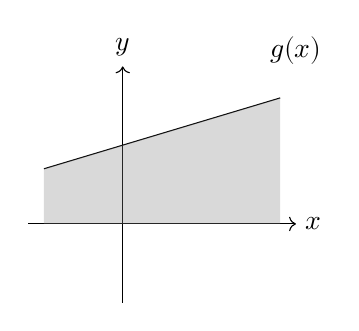
\begin{tikzpicture}
   \draw[->] (-1.2, 0) -- (2.2, 0) node[right] {$x$};
   \draw[->] (0, -1) -- (0, 2) node[above] {$y$};
   \node at (2.2,2.2) {\(g(x)\)};
   \draw[domain=-1:2, smooth, variable=\x] plot ({\x}, {0.3*\x+1});
   \fill [gray, domain=-1:2, variable=\x,opacity=0.3]
   (-1, 0)
   -- plot ({\x}, {\x*0.3+1})
   -- (2, 0)
   -- cycle;
 \end{tikzpicture}
\end{center}
where \(g(x)\gg f(x)\).

\(2\Rightarrow 3\): Suppose the structure \((G,<,+,\dots)\) is not stationary. Then there exist an \(H\succ G\)
and a \(H\)-definable function \(g:H\to H\) s.t. no \(G\)-definable map \(f:H\to H\) dominates \(g\)

Consider the following partial types over \(H\):
\begin{gather*}
p_1(x,y)=p_{+\infty}(x,y)\cup\{y<g(x)\}\\
p_2(x,y)=p_{+\infty}(x,y)\cup\{y>g(x)\}
\end{gather*}
To reach a contradiction, it is enough to prove that both of them are weak generic
in \((H,+)\times(H,+)\), and therefore \(p_+(x,y)\) is not stationary. We begin with \(p_1\).

Goal:
\begin{equation*}
(\bigwedge_{i=1}^mx>a_i)\wedge(\bigwedge_{i=1}^ny>f_i(x))\wedge y<g(x)
\end{equation*}
is weak generic in \((H,+)\times(H,+)\) where \(a_1,\dots,a_m\in G\) and \(f_1,\dots,f_n\) are functions
from \(H\) to \(H\) definable over \(G\).

Take \(a=\max(a_1,\dots,a_n)\) and \(f=\max(f_1,\dots,f_n)\) we can confine our attention to the
sets \(X\) of the form
\begin{equation*}
X=\{\la x,y\ra\in H\times H:x>a\wedge y>f(x)\wedge y<g(x)\}
\end{equation*}
where \(a\in G\) and \(f:H\to H\) is definable over \(G\). W.L.O.G., we can assume that \(f\) is
ultimately non-decreasing

Consider a map \(h:H\to H\) defined as follows: \(h(a)=f(2a)+a\) for each \(a\in H\). Since \(h\)
is \(G\)-definable, \(g\) dominates \(h\) \label{Problem5}.
\wu{
Non-stationarity means \(\forall x\in N\exists x<y\in N\) s.t. \(g(y)>h(y)\) and we can assume \(g\) is
ultimately increasing. Therefore we can define \(g'\) to be
\begin{equation*}
g'(x)=\min\{g(y):x<y\wedge g(y)>h(y)\}
\end{equation*}
Since \(h\) is non-decreasing, \(g'\) dominates \(h\).
}
Note that for each large enough \(M\in H\) the area
between the graphs of \(f\) and \(g\) in \(H\times H\) contains the square whose vertices are
\begin{equation*}
\la M,f(2M)\ra,\la M,f(2M)+M\ra, \la 2M,f(2M)\ra, \la 2M,f(2M)+M\ra
\end{equation*}
By Theorem \ref{3.3.4}, \(X\) is weak generic in \((H,+)\times(H,+)\). As a result, the type \(p_1\) is
weak generic in \((H,+)\times(H,+)\)

\(3\Rightarrow 1\): Take any definable \(f:G\to G\). We shall show that both \(p_f^+\) and \(p_f^-\) are
stationary weak generic types

By the o-minimality of \(G\), \(f\) is ultimately non-negative or ultimately non-positive. It is
easy to see that \(p_f^+\) is stationary iff \(p_{-f}^-\) is stationary and \(p_f^-\) is stationary
iff \(p_{-f}^+\) is stationary. Therefore, W.L.O.G, we can assume that \(f\) is ultimately
non-negative. Moreover, \(f\) is ultimately non-increasing or ultimately non-decreasing.
If \(f\) is ultimately non-increasing, then \(p_f^+=p_z^+\) and \(p_f^-=p_z^-\) where \(z:G\to G\) is
constantly equal to 0.
So we can assume that \(f\) is ultimately non-decreasing (this includes the constant case)

Consider definable sets:
\begin{align*}
A&=\{a\in G:(\exists b>a)(\forall c\in(a,b))f(c)-f(a)\le c-a\}\\
B&=\{a\in G:(\exists b>a)(\forall c\in(a,b))f(c)-f(a)>c-a\}
\end{align*}
Note that by the o-minimality of \(G\), we have that \(G=A\cup B\) and for some \(M\in G\)
either \((M,+\infty)\subseteq A\) or \((M,+\infty)\subseteq B\). Enlarge \(M\) in order to ensure that \(f\) is continuous
on \((M,+\infty)\)

\textbf{Case 1}: \((M,+\infty)\subseteq A\). Then \(f\) grows ``slowly'' on \((M,+\infty)\):
\begin{equation*}
(\forall a>M)(\exists b>0)(\forall c\in(0,b))f(a+c)\le f(a)+c\tag{\star}
\end{equation*}
By (\(\star\)) and the continuity of \(f\)
\begin{equation*}
(\forall a>M)(\forall c>0)f(a+c)\le f(a)+c\tag{\star\star}
\end{equation*}
Because if not, then the opposite holds: \((\exists a>M)(\exists c>0)f(a+c)>f(a)+c\).
Let \(C=\{c>0:f(a+c)>f(a)+c\}\) and \(c_0=\inf(C)\).
Assertion (\(\star\)) implies that \(c_0>0\). Since \(f\) is continuous at \(c_0\), \(c_0\notin C\).
Choose \(d>c_0\) s.t. \((c_0,d)\subseteq C\). Since \(c_0\notin C\), \(f(a+c_0)\le f(a)+c_0\). On the other
hand, by the continuity of \(f\) at \(a+c_0\), we have that \(f(a+c_0)\ge f(a)+c_0\).
Thus \(f(a+c_0)=f(a)+c_0\) and for every \(e\in(0,d-c_0)\) we have that
\begin{equation*}
f(a+c_0+e)>f(a)+c_0+e=f(a+c_0)+e
\end{equation*}
which implies that \(a+c_0\notin A\). But \(a+c_0\in(M,+\infty)\subseteq A\), a contradiction. So (\(\star\star\) holds)

For the sake of contradiction assume that \(p_f^+\) is not stationary. Then for some \(H\succ G\) and
\(H\)-definable \(g:H\to H\) we have that \(f\ll g\) and \(g\ll h\) for each \(G\)-definable \(h:H\to H\)
with \(f\ll h\).
\wu{
Use the same technique above. If \(p_f^+\) is not stationary, then there is some \(H\)-definable
function \(g\) s.t. both
\begin{gather*}
p_f^+(x,y)\cup\{y>g(x)\}\\
p_f^+(x,y)\cup\{y\le g(x)\}
\end{gather*}
are weak generic, which implies that \(f\ll g\ll h\) for each \(G\)-definable \(h:H\to H\)
with \(f\ll h\).
}
Since \(\lim_{x\to+\infty}(g(x)-f(x))=+\infty\), there exists an increasing
to \(+\infty\) \(G\)-definable function \(h:H\to H\) s.t. ultimately \(h\le g-f\) by \ref{3.4.4}.
Enlarging \(M\) we can assume that \(h\) is increasing on \((M,​+\infty)\).

Now fix any positive \(R\in H\) and find \(a>M\) with \(h(a)\ge 2R\). By (\(\star\star\)), we have
that \(f(a+R)\le f(a)+R\). So the area between the graphs of \(f\) and \(f+h\) contains the square
whose vertices are
\begin{equation*}
\la a,f(a)+R\ra,\la a,f(a)+2R\ra,\la a+R,f(a)+R\ra,\la a+R,f(a)+2R\ra
\end{equation*}
As \(R\) was arbitrary, we can use Theorem \ref{3.3.4} to conclude that the area between the
graphs of \(f\) and \(f+h\) is weak generic in \((H,+)\times(H,+)\). So \(f\ll f+h\) and
therefore \(g\ll f+h\), which contradicts the fact that ultimately \(g\ge f+h\). So the
type \(p_f^+\) is stationary

\textbf{Case 2}: \((M,+\infty)\subseteq B\).  Then \(f\) grows ``quickly'' on \((M,+\infty)\), which implies
that \(\lim_{x\to+\infty}f(x)=+\infty\). As in \ref{3.4.4} find a definable bijection \(f_1:G\to G\)
s.t. \(f_1(a)=f(a)\) for each \(a\in(M,+\infty)\). If \(g=f_1^{-1}\), then \(g\) grows ``slowly''
on \((M,+\infty)\) and from the previous case we know that the types \(p_g^+\) and \(p_g^-\) are
stationary. The proof is complete since
\(p_f^+(x,y)=p_{f_1}^+(x,y)=p_g^-(y,x)\) and \(p_f^-(x,y)=p_{f_1}^-(x,y)=p_g^+(x,y)\)
\end{proof}

\begin{corollary}[1.7.6 of \cite{van1998tame}]
\label{V1.7.6}
Let \(\cals_m\) be the boolean algebra of semilinear subsets of \(R^m\). Then \(\cals:=(\cals_m)_{m\in\N}\) is
an o-minimal structure on the ordered set \((R,<)\). Each function in \(\cals\) is piecewise affine,
more precisely, given a function \(f:A\to R\) in \(\cals\) with \(A\subseteq R^m\), there is a partition
of \(A\) into basic semilinear sets \(A_i\) (\(1\le i\le k\)) s.t. \(f|A_i\) is the restriction
to \(A_i\) of an affine function on \(R^m\), for each \(i\in\{1,\dots,k\}\)
\end{corollary}

\begin{examplle}[]
If \((G,<,+)\) is an o-minimal ordered group, then every definable function \(f:G\to G\) is
ultimately equal to \(f_q(x)+a\) for some \(a\in G\) and \(q\in\Q\) where \(f_q(x)=q\cdot x\)
(\ref{V1.7.6}) by considering \(G\) as a \(\Q\)-vector space. Below we list
all weak generic types in \((G,+)\times(G,+)\)
that are complete over \(G\) and contain the formula \(x>0\)
\begin{enumerate}
\item \(p_{-\infty}(x,y)\) and \(p_{+\infty}(x,y)\)
\item \(p_{f_q}^-(x,y)\) and \(p_{f_q}^+(x,y)\), \(q\in\Q\)
\item \(\{x>a:a\in G\}\cup\{y>q\cdot x:q\in\Q\wedge q<r\}\cup\{y<q\cdot x:q\in\Q\wedge q>r\}\), \(r\in\R\setminus\Q\)
\end{enumerate}
The structure \((G,<,+)\) is stationary since its elementary extensions are all linearly
bounded. Thus by Theorem \ref{3.4.7}, weak generic types of the form (1) and (2) are stationary.
\label{Problem7}
\end{examplle}

\subsection{Expansions of real closed fields}
\label{sec:org4b950dc}
In this section, \((R,<,+,\cdot,0,1,\dots)\) is an o-minimal expansion of an ordered
ring \((R,<,+,\cdot,-,0,1)\). Such a ring must be a real closed field. Since \((R,<,+,\cdot,0,1,\dots)\) is an
o-minimal expansion of the ordered group \((R,<,+)\), all results obtained in the previous
section apply

\begin{definition}[]
We call a structure \((R,<,+,\cdot,\dots)\) \textbf{polynomially bounded} if for every definable
function \(f:R\to R\) there is \(n\in\N^+\) s.t. \(\abs{f(x)}\le x^n\) for all sufficiently large \(x\in R\)
\end{definition}

\begin{remark}
\label{3.5.2}
If a real closed field \((R,<,+,\cdot,\dots)\) is polynomially bounded and o-minimal, then for every
definable \(f:R\to R\) with \(\lim_{x\to+\infty}f(x)=+\infty\) we can find \(n\in\N_+\) s.t. \(f(x)\ge\sqrt[n]{x}\)
for all sufficiently large \(x\in R\)
\end{remark}

\begin{proof}
We proceed as in the proof of \ref{3.4.4}. Since \(f\) is ultimately increasing, we are able to
find a definable bijection \(g:R\to R\) s.t. \(f(x)=g(x)\) for all sufficiently large \(x\in R\). We
know that the inverse map \(g^{-1}\) is ultimately dominated by the polynomial
function \(x\mapsto x^n\) for some \(n\in\N_+\). And this implies \(f(x)=g(x)\ge\sqrt[n]{x}\) for
sufficiently large \(x\)
\end{proof}

\begin{proposition}[2.6.1 of \cite{bochnak2013real}]
\label{B2.6.1}
Given a real closed field \(R\), let \(f\) be a semi-algebraic function (not necessarily
continuous) from \((a,+\infty)\subset R\) to \(R\). There exists \(r,c\in R\), \(r>a\), and \(p\in\N\), s.t.,
for every \(x\ge r\), we have \(\abs{f(x)}\le cx^p\). Moreover, if \(h\in R[X,Y]\) is a nonzero
polynomial, s.t. \(h(x,f(x))=0\) on \((a,+\infty)\), we can take \(p\) to be the degree of \(h\) w.r.t. \(X\)
\end{proposition}


Assume \((R,<,+,\cdot)\) is a pure real closed field. Since every definable map \(f:R\to R\) is
semi-algebraic, it follows from \ref{B2.6.1} that the
structure \((R,<,+,\cdot)\) is polynomially bounded.

\begin{corollary}[]
Every pure real closed field \((R,<,+,\cdot)\) is stationary and so are the weak generic
types \(p_f^-(x,y)\) and \(p_f^+(x,y)\) for each definable \(f:R\to R\)
\end{corollary}

\begin{proof}
Consider an arbitrary elementary extension \(S\) of \(R\) and any definable map \(f:S\to S\).
Since the real closed field \((S,<,+,\cdot)\) is polynomially bounded, there exists \(n\in\N_+\) s.t.
ultimately \(\abs{f(x)}\le x^n\). This gives us the stationary of the structure \((R,<,+,\cdot)\)
\end{proof}

On the other hand, the structure \((\R,<,+,\cdot,e^x)\) is not polynomially bounded but it is still an
o-minimal expansion of the ordered field of real numbers (\cite{Wilkie1996ModelCR})

\begin{definition}[]
Assume \((R,+,\cdot,0,1)\) is a field, \(f,g:R\to R\) and \(g(x)\neq 0\) for all sufficiently
large \(x\in R\). We write \(f\approx g\) iff
\begin{equation*}
\lim_{x\to+\infty}\frac{f(x)}{g(x)}=1
\end{equation*}
\end{definition}

\begin{lemma}[2.5.2 of \cite{bochnak2013real}]
\label{B2.5.2}
Let \(A\subset R\) be a semi-algebraic set and \(\varphi:A\to R\) a semialgebraic function. There exists a
nonzero polynomial \(f\in R[X,Y]\) s.t. for every \(x\in A\), \(f(x,\varphi(x))=0\).
\end{lemma}

\begin{lemma}[3.5.5]
\label{3.5.5}
Assume \((R,<,+,\cdot)\) is a pure real closed field. If a function \(f:R\to R\) is definable and
ultimately non-zero, then for some \(q\in\Q\) and \(c\in R\setminus\{0\}\) we have that \(f(x)\approx c\cdot x^q\)
\end{lemma}

\begin{proof}
Let \(S\) be an arbitrary \(\abs{R}^+\)-saturated elementary extension of \(R\). We can
find \(a\in S\) s.t. \(a>r\) for every \(r\in R\). Let
\begin{equation*}
T=\{s\in S:\abs{s}<r\text{ for some }r\in R\}
\end{equation*}
Then \(T\) is a convex subring of \(S\),
\begin{equation*}
T^*=\{s\in S:\frac{1}{r}<\abs{s}<r\text{ for some }r\in R\}
\end{equation*}
and \((T^*,\cdot)\) is a subgroup of the multiplicative group \((S^*,\cdot)\).

The quotient group \((S^*/T^*,*,\bone)\) may be ordered in the following way:
\begin{equation*}
s_1/T^*\le s_2/T^*\Leftrightarrow\frac{s_1}{s_2}\in T
\end{equation*}
We define a function \(\nu:S\to S^*/T^*\cup\{-\infty\}\) (where for every \(s\in S^*\), \(-\infty<s/T^*\)
and \((-\infty)* s/T^*=-\infty\)) as follows:
\begin{equation*}
\nu(s)=
\begin{cases}
-\infty&s=0\\
s/T^*&\text{otherwise}
\end{cases}
\end{equation*}
Then \(\nu\) is a valuation of the field \(S\), i.e., \(\forall x,y\in S\),
\begin{enumerate}
\setcounter{enumi}{0}
\item \(\nu(x\cdot y)=\nu(x)*\nu(y)\)
\item \(\nu(x+y)\le\max(\nu(x),\nu(y))\)

Suppose \(x,y\neq 0\) and \(\nu(x)\le\nu(y)\), then \(\frac{x}{y}\in T\), \(1+\frac{x}{y}\in T\) and
therefore \(\nu(x+y)\le\nu(y)\).
Since \(\frac{\frac{x}{y}}{\frac{x}{y}+1}\in T\), \(\frac{x}{x+y}\in T\) and so \(\nu(x+y)\ge\nu(y)\).
\item \(\nu(x)\neq\nu(y)\Rightarrow\nu(x+y)=\max(\nu(x),\nu(y))\)
\end{enumerate}


Since \(f\) is semi-algebraic, by Lemma \ref{B2.5.2}, there exists a
non-zero polynomial \(P(X,Y)\in R[X,Y]\) s.t. \(R\vDash\forall x(P(x,f(x))=0)\). So \(S\vDash\forall x(P(x,f(x))=0)\)
and, in particular, \(P(a,f(a))=0\). The polynomial \(P(X,Y)\) is of the form
\begin{equation*}
P(X,Y)=\sum_{i=1}^nr_i\cdot X^{k_i}\cdot Y^{l_i}
\end{equation*}
for some \(n\in\N_+\), \(r_i\in R\setminus\{0\}\) and \(k_i,l_i<\omega\) s.t. \(\la k_i,l_i\ra\neq\la k_j,l_j\ra\) for
every \(i\neq j\in\{1,\dots,n\}\). Thus
\begin{equation*}
0=\sum_{i=1}^nr_i\cdot a^{k_i}\cdot f(a)^{l_i}
\end{equation*}
and for some \(i\neq j\in\{1,\dots,n\}\) we have that
\begin{equation*}
\nu(r_i\cdot a^{k_i}\cdot f(a)^{l_i})=\nu(r_j\cdot a^{k_j}\cdot f(a)^{l_j})\neq-\infty
\end{equation*}
since \(f(a)\neq 0\) (if \(f(a)=0\), then \(f:R\to R\) would be ultimately equal to 0)

This implies that \(\nu(\frac{r_i}{r_j}\cdot a^{k_i-k_j}\cdot f(a)^{l_i-l_j})=\bone\)
and \(\nu(a^{k_i-k_j}\cdot f(a)^{l_i-l_j})=\bone\). So \(a^{k_i-k_j}\cdot f(a)^{l_i-l_j}\in T^*\). If \(l_i=l_j\),
then \(k_i\neq k_j\) and \(a^{k_i-k_j}\in T^*\), which implies that \(a\in T^*\), a contradiction.

So \(l_i\neq l_j\). Let \(q=-\frac{k_i-k_j}{l_i-l_j}\in\Q\) we obtain \(\frac{f(a)}{a^q}\in T^*\).
Therefore \(\frac{1}{r}<\abs{\frac{f(a)}{a^q}}<r\) for some \(r\in R\). If \(b\in S\) and \(b>a\),
then \(\tp(a/R)=\tp(b/R)\). Hence for every \(b>a\) we have
that \(\frac{1}{r}<\abs{\frac{f(b)}{b^q}}<r\) and consequently
\begin{equation*}
S\vDash\exists y\forall x(x>y\to\frac{1}{r}<\abs{\frac{f(x)}{x^q}}<r)
\end{equation*}
As \(R\prec S\), this implies that \(\frac{1}{r}<\abs{\frac{f(x)}{x^q}}<r\) for all sufficiently
large \(x\in R\). By the o-minimality of \(R\), for some \(c\in R\) with \(\frac{1}{r}\le\abs{c}\le r\)
we have that \(\lim_{x\to+\infty}\frac{f(x)}{x^q}=c\), which finishes the proof
\end{proof}

\begin{theorem}[3.5.6]
\label{3.5.6}
Assume \((R,<,+,\cdot)\) is a pure real closed field. Let
\begin{equation*}
f(x)=\sum_{i=1}^ma_i\cdot x^{p_i}\quad\text{ and }\quad g(x)=\sum_{j=1}^nb_j\cdot x^{q_j}
\end{equation*}
where \(m,n\in\N_+\), \(a_1,\dots,a_m,b_1,\dots,b_n\in R\), \(a_1,b_1>0\), \(p_1>\dots>p_m\in\Q\) and \(q_1>\dots>q_n\in\Q\). TFAE
\begin{enumerate}
\item \(f\ll f+g\)
\item \(q_1>\max(0,p_1-1)\)
\end{enumerate}
\end{theorem}

\begin{proof}
Goal: Ultimately, for each \(M\in R\), \(x^{p_1}+x^{q_1}\ge (x+M)^{p_1}+M\). Then
ultimately, \(x^{q_1}\ge k(M)\cdot x^{p_1-1}+M\) for some constant \(k\) relevant to \(M\).

We define a rate of growth \(gr(f)\) of a definable map \(f:R\to R\) as follows:
if \(f(x)\approx c\cdot x^q\) for some \(c\in R\setminus\{0\}\) and \(q\in\Q\), then \(gr(f)=q\) (Lemma \ref{3.5.5} implies
that \(gr(f)\) is well defined for each ultimately non-zero definable function \(f:R\to R\))
and \(gr(f)=0\) otherwise.
\begin{equation*}
gr(f)=
\begin{cases}
q&\exists c\in R\setminus\{0\}\exists q\in\Q\text{ s.t. }f(x)\approx c\cdot x^q\\
0&\text{otherwise}
\end{cases}
\end{equation*}
Then \(gr(f\cdot g)=gr(f)+gr(g)\) and \(gr(f+g)=\max(gr(f),gr(g))\) provided \(gr(f)\neq gr(g)\)

First, we prove that \((x+c)^q-x^q\approx c\cdot q\cdot x^{q-1}\) for every \(c\in R\setminus\{0\}\) and \(q\in\Q_+\).

Let \(q=\frac{p}{p'}\) where \(p,p'\in\Z_+\). For each \(x\in R_+\) let \(\Delta(x)=(x+c)^q-x^q\) and note
that \(\lim_{x\to+\infty}(\Delta(x)\cdot x^{-q})=0\), which implies that \(gr(\Delta(x))<q\).
Since \((x+c)^p=(\Delta(x)+x^q)^{p'}\), we have that
\begin{equation*}
\sum_{i=0}^p\binom{p}{i}\cdot x^i\cdot c^{p-i}=\sum_{i=0}^{p'}\binom{p'}{i}\cdot\Delta(x)^i\cdot(x^q)^{p'-i}
\end{equation*}
and
\begin{equation*}
L(x)=\sum_{i=0}^{p-1}\binom{p}{i}\cdot x^i\cdot c^{p-i}=\sum_{i=1}^{p'}\binom{p'}{i}\cdot\Delta(x)^i\cdot(x^q)^{p'-i}=R(x)
\end{equation*}
Obviously, \(gr(L(x))=gr(\binom{p}{p-1}\cdot x^{p-1}\cdot c)=p-1\). On the other hand,
since \(gr(\Delta(x))<q\), we have that
\begin{equation*}
gr(R(x))=gr(\binom{p'}{1}\cdot\Delta(x)\cdot(x^q)^{p'-1})=gr(\Delta(x))+q\cdot(p'-1)
\end{equation*}
Thus \(gr(\Delta(x))=p-1-q\cdot(p'-1)=q-1\) and \(\Delta(x)\approx c\cdot q\cdot x^{q-1}\)

\(1\Rightarrow 2\): We see that \(q_1>0\) because otherwise for some \(c\in R\) we would have
that \(\abs{g(x)}\le c\) for large \(x\in R\) and consequently \(f\sim f+g\). Now if \(p_1-1\le 0\),
then \(q_1>p_1-1\), which finishes the proof. So we can assume \(p_1>1\)

We know that \(f(x)<f(x)+g(x)\) for all sufficiently large \(x\in R\) and the set
\begin{equation*}
A_f^{f+g}=\{\la x,y\ra\in R\times R:x> 0\wedge f(x)<y\wedge y<f(x)+g(x)\}
\end{equation*}
is weak generic in \((R\times R,+)\). By Theorem \ref{3.3.4}, for every \(M\in R_+\) there
exist \(x_M,y_M\in R\) s.t.
\begin{equation*}
\{\la x,y\ra\in R\times R:x_M<x\wedge x<x_M+M\wedge y_M<y\wedge y<y_M+M\}\subseteq A_f^{f+g}
\end{equation*}
This implies that \(f(x_M)+g(x_M)\ge f(x_M+M)+M\) for all sufficiently large \(M\in R\). Note
that \(\lim_{M\to+\infty}x_M=+\infty\)

Put \(M_0=\frac{b_1+1}{a_1p_1}\). Then still for all sufficiently large \(M\in R\) we have
that \(f(x_M)+g(x_M)\ge f(x_M+M_0)+M_0\) and by the o-minimality
of \((R,<,+,\cdot)\), \(f(x)+g(x)\ge f(x+M_0)+M_0\) for all sufficiently large \(x\in R\). So ultimately
\begin{equation*}
\sum_{i=1}^ma_i\cdot x^{p_i}+\sum_{j=1}^nb_j\cdot x^{q_j}\ge M_0+\sum_{i=1}^ma_i\cdot(x+M_0)^{p_i}
\end{equation*}
and
\begin{equation*}
\sum_{j=1}^nb_j\cdot x^{q_j}\ge M_0+\sum_{i=1}^ma_i\cdot((x+M_0)^{p_i}-x^{p_i})
\end{equation*}
Finally, comparing the ingredients of the sums with the biggest value of gr we see that
ultimately
\begin{equation*}
b_1\cdot x^{q_1}\ge a_1\cdot((x+M_0)^{p_1}-x^{p_1})\approx a_1\cdot M_0\cdot p_1\cdot x^{p_1-1}=(b_1+1)\cdot x^{p_1-1}
\end{equation*}
Hence \(q_1>p_1-1\)

\(2\Rightarrow 1\): Fix \(M\in R_+\). Since \(q_1>\max(0,p_1-1)\), similar as above, we can show that for all
sufficiently large \(x\in R\)
\begin{equation*}
\sum_{i=1}^ma_i\cdot x^{p_i}+\sum_{j=1}^nb_j\cdot x^{q_j}\ge M+\sum_{i=1}^ma_i\cdot(x+M)^{p_i}
\end{equation*}
This means that ultimately \(f(x)+g(x)\ge f(x+M)+M\). Choose \(x_M\in R_+\) satisfying the latter
inequality and s.t. \(f\) and \(g\) are increasing on the interval \((x_M,+\infty)\). Then
for \(y_M=f(x_M+M)\) we have that
\begin{equation*}
\{\la x,y\ra\in R\times R:x_M<x\wedge x<x_M+M\wedge y_M<y\wedge y<y_M+M\}\subseteq A^{f+g}_f
\end{equation*}
\end{proof}

\begin{examplle}[3.5.7]
\label{3.5.7}
Let \((R,<,+,\cdot)\) be a pure real closed field and for \(a\in\R_+\setminus\Q\) let
\begin{equation*}
p(x,y)=\{x>r:r\in R\}\cup\{y>x^q:a>q\in\Q\}\cup\{y<x^q:a<q\in\Q\}
\end{equation*}
We shall prove that \(p\) is a stationary (complete) weak generic type in the group \((R,+)\times(R,+)\)
and \(p\) is not of the form \(p_f^-\) or \(p_f^+\) for any definable \(f:R\to R\)

The weak genericity of \(p\) follows from Theorem \ref{3.5.6}. Indeed, the set
\begin{equation*}
\{\la x,y\ra\in R\times R:x>r\wedge y>x^{q_1}\wedge y<x^{q_2}\}
\end{equation*}
is weak generic in \((R,+)\times(R,+)\) since \(q_2>\max(0,q_1-1)\)

The stationary (and the completeness) of \(p\) follows from Lemma \ref{3.5.5}. Namely, if \(p\)
were non-stationary, then for some \(S\succ R\) and definable \(f:S\to S\) we would have that
ultimately \(f(x)>x^q\) for each \(q\in\Q\cap(-\infty,a)\) and ultimately \(f(x)<x^q\) for
each \(q\in\Q\cap(a,+\infty)\). By Lemma \ref{3.5.5}, \(f(x)\approx c\cdot x^q\) for some \(q\in\Q\) and \(c\in S_+\)
(\(c>0\) since \(f\) is ultimately increasing). Assume that \(q>a\) and take any \(r\in\Q\cap(a,q)\).
Then ultimately \(f(x)>x^r\) (since \(q>r\)). On the other hand, ultimately \(f(x)<x^r\)
(since \(r\in\Q\cap(a,+\infty)\)). If \(q<a\), then we reach a contradiction in a similar way. As a
result, \(p\) is stationary (and complete) \label{Problem6}

Suppose \(p(x,y)=p'(x,y)\) for some definable function \(f:R\to R\) and a type
\(p'(x,y)\in\{p_f^-(x,y),p_f^+(x,y)\}\). Then \(f(x)\approx c\cdot x^q\) for some \(q\in\Q\) and \(c\in R_+\).
W.L.O.G., \(q>a\). Take any \(r\in\Q\cap(a,q)\). Then \((y<x^r)\in p(x,y)\) and \((y>x^r)\in p'(x,y)\), a
contradiction.
\end{examplle}

\begin{examplle}[3.5.8]
\label{3.5.8}
Let \((R,<,+,\cdot,\dots)\) be an o-minimal polynomially bounded expansion of a real closed
field \((R,<,+,\cdot)\) and for \(q_0\in\Q_+\) let
\begin{equation*}
p(x,y)=\{x>r:r\in R\}\cup\{y>r\cdot x^{q_0}:r\in R\}\cup\{y<x^q:q_0<q\in\Q\}
\end{equation*}
We shall prove that \(p\) is a non-stationary complete weak generic type in the
group \((R,+)\times(R,+)\)

It \(p\) were not complete, then we could find a definable function \(f:R\to R\) s.t.
ultimately \(f(x)<x^q\) for each \(q\in\Q\cap(q_0,+\infty)\) and ultimately \(f(x)>r\cdot x^{q_0}\) for
each \(r\in R\) (thus \(\lim_{x\to+\infty}\frac{f(x)}{x^{q_0}}=+\infty\)). By Remark
\ref{3.5.2}, \(\frac{f(x)}{x^{q_0}}\ge\sqrt[n]{x}\) for some \(n\in\N_+\) and all sufficiently
large \(x\in R\). But then ultimately \(f(x)\ge x^{q_0+\frac{1}{n}}\), a contradiction.

To obtain non-stationarity of \(p\), let \(S\) be an \(\abs{R}^+\)-saturated elementary extension
of \(R\) and choose any \(a\in S\) s.t. \(a>r\) for every \(r\in R\). Then
\begin{equation*}
\{x>r:r\in R\}\cup\{y>r\cdot x^{q_0}:r\in R\}\cup\{y<x^q:q_0<q\in\Q\}\cup\{y<a\cdot x^{q_0}\}
\end{equation*}
and
\begin{equation*}
\{x>r:r\in R\}\cup\{y>r\cdot x^{q_0}:r\in R\}\cup\{y<x^q:q_0<q\in\Q\}\cup\{y>a\cdot x^{q_0}\}
\end{equation*}
are two distinct extensions of \(p\) to weak generic types in \((S,+)\times(S,+)\)
\end{examplle}
In \(\RCF\), we can approximate the definable function .

\subsubsection{Weak generic types in \texorpdfstring{\((\R,+)\times(\R,+)\)}{R^2}}
\label{sec:org8f8f712}
Now we give a description of complete (over \(\R\)) weak generic types in the
group \((\R,+)\times(\R,+)\) derived in the theory \(\Th(\R,<,+,\cdot)\).

Let \(S\) be a \((2^{\aleph_0})^+\)-saturated elementary extension of the field of reals.
Choose \(a\in S\) s.t. \(a>r\) for every \(r\in\R\). Let \(b_0\in S\) be s.t. \(b_0\neq\sum_{i=1}^nr_i\cdot a^{q_i}\)
for all \(n\in\N_+\), \(r_i\in\R\) and \(q_i\in\Q\) (in this case we say that \(b_0\) is non-polynomial over
\(a\)). We describe a recursive procedure of defining \(b_1,b_2,\dots\in S\setminus\{0\}\), \(r_1,r_2,\dots\in\R\setminus\{0\}\)
and \(q_1,q_2,\dots\in\Q_+\) so that \(q_1>q_2>\dots\) and \(b_n=b_0-r_1\cdot a^{q_1}-\dots-r_n\cdot a^{q_n}\) for
every \(n\in\N_+\).

First we define \(b_1,r_1\) and \(q_1\). We consider two cases, depending on whether \(b_0\) is
positive or negative.

\begin{itemize}
\item \textbf{Case P}. \(b_0>0\). Consider the following subsets of \(\Q_+\):
\begin{align*}
A&=\{q\in\Q_+:(\forall r\in\R_+)b_0>r\cdot a^q\}\\
B&=\{q\in\Q_+:(\forall r\in\R_+)b_0<r\cdot a^q\}
\end{align*}
The sets \(A\) and \(B\) are disjoint and there is a unique \(c\in\R_{\ge 0}\cup\{+​\infty\}\)
s.t. \(A\subseteq(0,c]\), \(B\subseteq[c,+\infty)\) and \(\Q_+\cup\{c\}=A\cup B\cup\{c\}\). We
define \(b_1,r_1,q_1\) only in the case where the following condition holds:
\begin{equation*}
c\in\Q_+,A=\Q_+\cap(0,c),B=\Q_+\cap(c,+\infty)\tag{\(\dagger\)}
\end{equation*}
Otherwise the procedure stops and no \(b_1,r_1,q_1\) are defined

If (\(\dagger\)) holds, then we put \(q_1=c\). We have that \(r'\cdot a^{q_1}<b_0<r''\cdot a^{q_1}\) for
some \(r'<r''\in\R_+\). Since the ordering \((\R,<)\) is Dedekind complete, there exists a
unique \(r\in\R_+\) s.t. for every \(r',r''\in\R_+\) with \(r'<r<r''\) we have
that \(r'\cdot a^{q_1}<b_0<r''\cdot a^{q_1}\). We put \(r_1=r\) and \(b_1=b_0-r_1\cdot a^{q_1}\).

\item \textbf{Case N}. \(b_0<0\). Here we proceed similarly. Consider the following subsets of \(\Q_+\):
\begin{align*}
&A=\{q\in\Q_+:(\forall r\in\R_-)b_0<r\cdot a^q\}\\
&B=\{q\in\Q_+:(\forall r\in\R_-)b_0>r\cdot a^q\}
\end{align*}
The sets \(A\) and \(B\) are disjoint and there is a unique \(c\in\R_{\ge 0}\cup\{+\infty\}\)
s.t. \(A\subseteq(0,c]\), \(B\subseteq[c,+\infty)\) and \(\Q_{​+}\cup\{c\}=A\cup B\cup\{c\}\). We define \(b_1,r_1\) and \(q_1\) only in
the case where (\(\dagger\)) holds. Otherwise the procedure stops and no \(b_1,r_1\) and \(q_1\) are
defined.

If (\(\dagger\)) holds, then we put \(q_1=c\). We have that \(r'\cdot a^{q_1}<b_0<r''\cdot a^{q_1}\) for
some \(r'<r''\in\R_-\). Since the ordering \((\R,<)\) is Dedekind complete, there exists a
unique \(r\in\R_-\) s.t. for every \(r',r''\in\R_-\) with \(r'<r<r''\) we have
that \(r'\cdot a^{q_1}<b_0<r''\cdot a^{q_1}\). We put \(r_1=r\) and \(b_1=b_0-r_1\cdot a^{q_1}\).
\end{itemize}

\begin{center}
  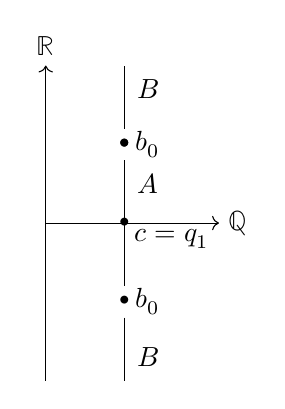
\begin{tikzpicture}
    \draw[->] (0, 0) -- (2.2, 0) node[right] {$\mathbb{Q}$};
    \draw[->] (0, -2) -- (0, 2) node[above] {$\mathbb{R}$};
    \node at (1.3,1) {\(b_{0}\)};
    \node at (1.3,-1) {\(b_{0}\)};
    \node at (1,1) {\textbullet};
    \node at (1,1) {\textbullet};
    \node at (1,0) {\textbullet};
    \node at (1,-1) {\textbullet};
    \node at (1.3,0.5) {\(A\)};
    \node at (1.6,-0.2) {\(c=q_1\)};
    \node at (1.3,1.7) {\(B\)};
    \node at (1.3,-1.7) {\(B\)};
    \draw[-] (1,0.8) -- (1,-0.8);
    \draw[-] (1,1.2) -- (1,2);
    \draw[-] (1,-1.2) -- (1,-2);
  \end{tikzpicture}
\end{center}

Suppose  \(b_i,r_i\) and \(q_i\) have been defined so that \(b_i\neq 0\). Again we consider two cases,
depending on whether \(b_i\) is positive or negative.

\begin{itemize}
\item \textbf{Case P}. \(b_i>0\). We define the sets \(A,B\) and \(c\in\R_{\ge 0}\cup\{+\infty\}\) as in the case of \(b_0>0\).
Again, if (\(\dagger\)) fails, then the procedure stops and \(b_j,r_j,q_j\) are not defined for
any \(j>i\). If (\(\dagger\)) holds, then we put \(q_{i+1}=c\) and define \(r_{i+1}\), \(b_{i+1}\)
analogously as in the case of \(b_0\).

\item \textbf{Case N}. \(b_i<0\). Similar.
\end{itemize}

If \(b_1,\dots,b_i,q_1,\dots,q_i\) and \(r_1,\dots,r_i\) are defined, then \(q_1>\dots>q_i\). We shall only prove
that \(q_1>q_2\). We have that
\begin{equation*}
b_2=b_1-r_2\cdot a^{q_2}=b_0-r_1\cdot a^{q_1}-r_2\cdot a^{q_2}
\end{equation*}
W.L.O.G., we can assume that \(r_2>0\). Choose any real number \(r\in(0,r_2)\).
Then \(b_1>r\cdot a^{q_2}\). If \(q_1\le q_2\), then also \(b_1>r\cdot a^{q_1}\) and
consequently \(b_0=b_1+r_1\cdot a^{q_1}>(r_1+r)\cdot a^{q_1}\), which contradicts the definition of \(r_1\).
Hence \(q_1>q_2\).

Secondly, note that \(b_k\neq 0\) for every \(k\in\{1,\dots,i\}\). Otherwise we would have that
\begin{equation*}
b_k=b_0-r_1\cdot a^{q_1}-\dots-r_n\cdot a^{q_n}=0
\end{equation*}
and \(b_0\) would be polynomial over \(a\), a contradiction.

Now we are able to give a description of complete weak generic types in the
group \((\R,+)\times(\R,+)\) (which implies that \(b_0\) is non-polynomial over \(a\)) and \(a>0\)
(hence \(a>r\) for every \(r\in\R\)). Denote the type \(\tp(\la a,b_0\ra/\R)\) by \(p(x,y)\) and note
that \(\{x>r:r\in\R\}\subseteq p(x,y)\).

\begin{itemize}
\item \textbf{Case A}. Assume that no \(b_i\) are defined for \(i>0\). This happens only if (\(\dagger\)) fails. We
shall consider one by one all possible cases. It turns out that each of these cases determines
uniquely the weak generic type \(\tp(\la a,b_0\ra/\R)\).

First, we consider the situation where \(b_0>0\). Let \(A,B\) be as in Case P.
\begin{itemize}
\item \textbf{Case 1}. \emph{\(A=\Q_+\cap(0,c)\) and \(B=\Q_+\cap(c,+\infty)\) for some \(c\in\R_+\setminus\Q\)}.

Then \(p(x,y)\) is the only extension of the type
\begin{equation*}
\{x>r:r\in\R\}\cup\{y>x^q:q\in\Q\cap(0,c)\}\cup\{y<x^q:q\in\Q\cap(c,+\infty)\}
\end{equation*}
to a complete weak generic type over \(\R\). Every weak generic type of this form is
stationary. (Example \ref{3.5.7})
\item \textbf{Case 2}. \emph{\(A=\Q_+\cap(0,q]\) and \(B=\Q_+\cap(q,+\infty)\) for some \(q\in\Q_+\).}

Then \(p(x,y)\) is the only extension of the type
\begin{equation*}
\{x>r:r\in\R\}\cup\{y>r\cdot x^q:r\in\R_+\}\cup\{y<x^{q'}:q'\in\Q\cap(q,+\infty)\}
\end{equation*}
to a complete weak generic type over \(\R\). Every weak generic type of this form is
non-stationary. (Example \ref{3.5.8})
\item \textbf{Case 3.} \emph{\(A=\Q_+\cap(0,q)\) and \(B=\Q_+\cap[q,+\infty)\) for some \(q\in\Q_+\)}.

Then \(p(x,y)\) is the only extension of the type
\begin{equation*}
\{x>r:r\in\R\}\cup\{y>x^{q'}:q'\in\Q\cap(0,q)\}\cup\{y<r\cdot x^q:r\in\R_+\}
\end{equation*}
to a complete weak generic type over \(\R\). Every weak generic type of this form is
non-stationary.
\item \textbf{Case 4}. \emph{\(A=\emptyset\) and \(B=\Q_+\)}.

Since \(p(x,y)\) is weak generic and \(b_0>0\), we also have that \(b_0>r\) for
every \(r\in\R\). Therefore \(p(x,y)=p_z^+(x,y)\) where \(z:\R\to\R\), \(z(r)=0\) for all \(r\in\R\).
By Theorem \ref{3.4.7}, \(p(x,y)\) is stationary.
\item \textbf{Case 5}. \emph{\(A=\Q_+\) and \(B=\emptyset\).}

Then \(p(x,y)=p_+(x,y)\). By Theorem \ref{3.4.7}, \(p(x,y)\) is
stationary.
\end{itemize}
If \(b_0<0\), then we get the following cases.
\begin{itemize}
\item \textbf{Case 1'}. \emph{\(A=\Q_+\cap(0,c)\) and \(B=\Q_+\cap(c,+\infty)\) for some \(c\in\R_+\setminus\Q\).}

Then \(p(x,y)\) is the only extension of the type
\begin{equation*}
\{x>r:r\in\R\}\cup\{y<-x^q:q\in\Q\cap(0,c)\}\cup\{y>-x^q:q\in\Q\cap(c,+\infty)\}
\end{equation*}
to a complete weak generic type over \(\R\).
\item \textbf{Case 2'}. \emph{\(A=\Q_+\cap(0,q]\) and \(B=\Q_+\cap(q,+\infty)\) for some \(q\in\Q_+\).}

Then \(p(x,y)\) is the only extension of the type
\begin{equation*}
\{x>r:r\in\R\}\cup\{y<r\cdot x^q:r\in\R_-\}\cup\{y>-x^{q'}:q'\in\Q\cap(q,+\infty)\}
\end{equation*}
to a complete weak generic type over \(\R\).
\item \textbf{Case 3'.} \emph{\(A=\Q_+\cap(0,q)\) and \(B=\Q_+\cap[q,+\infty)\) for some \(q\in\Q_+\)}.

Then \(p(x,y)\) is the only extension of the type
\begin{equation*}
\{x>r:r\in\R\}\cup\{y<-x^{q'}:q'\in\Q\cap(0,q)\}\cup\{y>r\cdot x^q:r\in\R_-\}
\end{equation*}
to a complete weak generic type over \(\R\).
\item \textbf{Case 4'}. \emph{\(A=\emptyset\) and \(B=\Q_+\).}

Since \(p(x,y)\) is weak generic and \(b_0<0\), we also have
that \(b_0<r\) for every \(r\in\R\). Therefore \(p(x,y)=p_z^-(x,y)\) where \(z:\R\to\R\) is
constantly equal to 0.
\item \textbf{Case 5'}. \emph{\(A=\Q_+\) and \(B=\emptyset\)}.

Then \(p(x,y)=p_{-\infty}(x,y)\)
\end{itemize}
\item \textbf{Case B}. Now assume that for \(a\) and \(b_0\) with \(\tp(\la a,b_0\ra/\R)\) weak generic the
procedure breaks down at some finite step so that \(b_i,r_i\) and \(q_i\) are defined only
for \(i\in\{1,\dots,n\}\). This means that in the condition (\(\dagger\)) fails at step \(n\).
Let \(f(x)=\sum_{i=1}^nr_i\cdot x^{q_i}\) and recall that \(r_i\in\R\setminus\{0\}\), \(q_i\in\Q_+\) and \(q_1>\dots>q_n\).

First we consider the situation where \(b_n>0\). Let \(A,B\) be as in Case P.
\begin{itemize}
\item \textbf{Case 1}. \emph{\(A=\Q_+\cap(0,c)\) and \(B=\Q_+\cap(c,+\infty)\) for some \(c\in\R_+\setminus\Q\).}

Then \(p(x,y)\) is the only extension of the type
\begin{align*}
r(x,y)=&\{x>r:r\in\R\}\cup\{y-f(x)>x^q:q\in\Q\cap(0,c)\}\cup\\
&\{y-f(x)<x^q:q\in\Q\cap(c,+\infty)\}
\end{align*}
to a complete weak generic type over \(\R\). Moreover, \(c>q_1-1\) and \(c<q_n\).
\wu{
For each \(p_1\in\Q\cap(c,+\infty)\) and \(p_2\in\Q\cap(0,c)\), ultimately, for each \(M\in\R_+\), we want
\(x^{p_1}+x^{q_1}\ge(x+M)^{q_1}+(x+M)^{p_2}+M\), which is equivalent to
\(x^{p_1}\ge k(M)x^{q_1-1}\) and \(p_1>q_1-1\). Therefore \(c>q_1-1\).
}
\label{Problem8}
\item \textbf{Case 2}. \emph{\(A=\Q_+\cap(0,q]\) and \(B=\Q_+\cap(q,+\infty)\) for some \(q\in\Q_+\).}

Then \(p(x,y)\) is the only extension of the type
\begin{gather*}
\{x>r:r\in\R\}\cup\{y-f(x)>r\cdot x^q:r\in\R_+\}\cup\\
\{y-f(x)<x^{q'}:q'\in\Q\cap(q,+\infty)\}
\end{gather*}
to a complete weak generic type over \(\R\). Moreover, \(q\ge q_1-1\)
\wu{
since \(q'>q_1-1\) for any \(q'>q\)
}
and \(q<q_n\).
If \(q=q_1-1\), then \(p(x,y)\) is stationary (since then \(p(x,y)=p_f^+(x,y)\)).
If \(q>q_1-1\), then \(p(x,y)\) is non-stationary. (Example \ref{3.5.8})
\item \textbf{Case 3}. \emph{\(A=\Q_+\cap(0,q)\) and \(B=\Q_+\cap[q,+\infty)\) for some \(q\in\Q_+\).}

Then \(p(x,y)\) is the only extension of the type
\begin{gather*}
\{x>r:r\in\R\}\cup\{y-f(x)>x^{q'}:q'\in\Q\cap(0,q)\}\cup\\
\{y-f(x)<r\cdot x^q:r\in\R_+\}
\end{gather*}
to a complete weak generic type over \(\R\). Moreover, \(q>q_1-1\) and \(q<q_n\). Every weak
generic type of this form is non-stationary.
\item \textbf{Case 4}. \emph{\(A=\emptyset\) and \(B=\Q_+\).}

Then \(p(x,y)\) is the only extension of the type
\begin{equation*}
\{x>r:r\in\R\}\cup\{y-f(x)>0\}\cup\{y-f(x)<x^q:q\in\Q_+\}
\end{equation*}
to a complete weak generic type over \(\R\). Moreover, \(q_1\le 1\) and \(p(x,y)=p_f^+(x,y)\). By
Theorem \ref{3.4.7}, \(p(x,y)\) is stationary.
\item \textbf{Case 5.} \emph{\(A=\Q_+\) and \(B=\emptyset\).}

Then \(p(x,y)\) contains the following set of formulas
\begin{equation*}
\{x>r:r\in\R\}\cup\{y-f(x)>x^q:q\in\Q_+\}
\end{equation*}
Take any rational \(q>q_1\). Then \((y-f(x)>x^q)\in p(x,y)\), which implies
that \(b_0-f(a)>a^q\). Hence
\begin{equation*}
b_0>a^q+\sum_{i=1}^n\cdot a^{q_i}
\end{equation*}
which contradicts the choice of \(q_1\). So case 5 can not hold.
\end{itemize}
If \(b_n<0\), then we get the following cases: Let \(A,B\) be as in Case N.
\begin{itemize}
\item \textbf{Case 1'}. \emph{\(A=\Q_+\cap(0,c)\) and \(B=\Q_+\cap(c,+\infty)\) for some \(c\in\R_+\setminus\Q\).}

Then \(p(x,y)\) is the only extension of the type
\begin{gather*}
\{x>r:r\in\R\}\cup\{y-f(x)<-x^q:q\in\Q\cap(0,c)\}\cup\\
\{y-f(x)>-x^q:q\in\Q\cap(c,+\infty)\}
\end{gather*}
to a complete weak generic type over \(\R\). Moreover, \(c>q_1-1\) and \(c<q_n\).
\item \textbf{Case 2'}. \emph{\(A=\Q_+\cap(0,q]\) and \(B=\Q_+\cap(q,+\infty)\) for some \(q\in\Q_+\).}

Then \(p(x,y)\) is the only extension of the type
\begin{gather*}
\{x>r:r\in\R\}\cup\{y-f(x)<r\cdot x^q:r\in\R_-\}\cup\\
\{y-f(x)>-x^{q'}:q'\in\Q\cap(q,+\infty)\}
\end{gather*}
to a complete weak generic type over \(\R\). Moreover, \(q\ge q_1-1\) and \(q<q_n\).
If \(q=q_1-1\), then \(p(x,y)=p_f^-(x,y)\).
\item \textbf{Case 3'}. \emph{\(A=\Q_+\cap(0,q)\) and \(B=\Q_+\cap[q,+\infty)\) for some \(q\in\Q_+\).}

Then \(p(x,y)\) is the only extension of the type
\begin{gather*}
\{x>r:r\in\R\}\cup\{y-f(x)<-x^{q'}:q'\in\Q\cap(0,q)\}\cup\\
\{y-f(x)>r\cdot x^q:r\in\R_-\}
\end{gather*}
to a complete weak generic type over \(\R\). Moreover, \(q>q_1-1\) and \(q<q_n\).
\item \textbf{Case 4'}. \emph{\(A=\emptyset\) and \(B=\Q_+\).}

Then \(p(x,y)\) is the only extension of the type
\begin{equation*}
\{x>r:r\in\R\}\cup\{y-f(x)<0\}\cup\{y-f(x)>-x^q:q\in\Q_+\}
\end{equation*}
to a complete weak generic type over \(\R\). Moreover, \(q_1\le 1\) and \(p(x,y)=p_f^-(x,y)\).
\item \textbf{Case 5'}. \emph{\(A=\Q_+\) and \(B=\emptyset\).}

Impossible.
\end{itemize}
\item \textbf{Case C}. Now assume that for \(a\) and \(b_0\) with \(\tp(\la a,b_0\ra/\R)\) weak generic the
procedure never stops and we have defined \(b_i,r_i\) and \(q_i\) for all \(i\in\N_+\). Recall
that \(b_i\in S\setminus\{0\}\), \(r_i\in\R\setminus\{0\}\), \(q_i\in\Q_+\), \(q_1>q_2>\dots\) and for every \(i\in\N_+\) we have
that \(b_i=b_0-r_1\cdot a^{q_1}-\dots-r_i\cdot a^{q_i}\).

Let \(f\) be the formal power series \(\sum_{i=1}^{+\infty}r_i\cdot x^{q_i}\) and for each \(n\in\N\)
let \(f_n(x)=\sum_{i=1}^nr_i\cdot x^{q_i}\) (in particular, \(f_0=0\)). We shall prove that the
type \(p(x,y)=\tp(\la a,b_0\ra/\R)\) is the only extension of the type \(p_f(x,y)\) to a complete
weak generic type over \(\R\) where the type \(p_f(x,y)\) is defined as follows:
\begin{gather*}
  \{x>r:r\in\R\}\cup\{y-f_n(x)>r'\cdot x^{q_{n+1}}:n\in\N\wedge r'\in\R\wedge r'<r_{n+1}\}\cup\\
  \{y-f_n(x)<r''\cdot x^{q_{n+1}}:n\in\N\wedge r''\in\R\wedge r''>r_{n+1}\}
\end{gather*}
Then \(p_f(x,y)\subseteq p(x,y)\). Assume that the weak generic types \(p(x,y)=\tp(\la a,b_0\ra/\R)\)
and \(p'(x,y)=\tp(\la a',b_0'\ra/\R)\) (\(a',b_0'\in S\)) are two distinct extensions of the
type \(p_f(x,y)\) (hence \(\la a,b_0\ra\) and \(\la a',b_0'\) produce the same formal power
series \(f=\sum_{i=1}^{+\infty}r_i\cdot x^{q_i}\)). W.L.O.G., we can assume that \(a=a'\).

Since \(p\neq p'\), there exists a definable (and thus semi-algebraic) function \(g:\R\to\R\)
s.t. \((y<g(x))\in p\) and \((y>g(x))\in p'\). We shall prove that the map \(g\) can be replaced
with the map of the form \(h(x)=\sum_{i=1}^ns_i\cdot x^{p_i}\) where \(n\in\N_+\), \(s_i\in\R\) and \(p_i\in\Q\).

Random links: \href{http://homepages.math.uic.edu/\~jan/mcs563s14/puiseux.pdf}{link1}

We know that \(g\) has a Puiseux expansion of the form
\begin{equation*}
g(x)=\sum_{i=k}^{+\infty}c_i\cdot x^{\frac{-i}{d}}\tag{\star}
\end{equation*}

where \(k\in\Z\), \(d\in\Z_+\) and \(c_i\in\R\) for \(i\ge k\). Equality (\(\star\)) holds for all sufficiently
large \(x\in\R\). One can prove that for some \(M\in\R_+\) we obtain ultimately
\begin{equation*}
\abs{g(x)-\sum_{i=k}^{-1}c_i\cdot x^{\frac{-i}{d}}}\le M
\end{equation*}
Let \(h(x)=\sum_{i=k}^{-1}c_i\cdot x^{\frac{-i}{d}}\). Then still \((y<h(x))\in p\)
and \((y>h(x))\in p'\), which means that \(b_0<h(a)\) and \(b_0'>h(a)\).

Choose unique \(n\in\N_+\), \(s_i\in\R\setminus\{0\}\) and \(p_i\in\Q_+\) s.t.
(ultimately) \(h(x)=\sum_{i=1}^ns_i\cdot x^{p_i}\) and \(p_1>\dots>p_n\). Then for each \(i\in\{1,\dots,n\}\) we have
that \(p_i=q_i\) and \(s_i=r_i\). We shall only prove that \(p_1=q_1\) and \(s_1=r_1\).

In order to show that \(p_1=q_1\), we shall consider several possible cases.
\begin{itemize}
\item If \(p_1<q_1\) and \(r_1>0\), then
\begin{equation*}
h(a)=s_1\cdot a^{p_1}+\sum_{i=2}^ns_i\cdot a^{p_i}<\frac{r_1}{2}\cdot a^{q_1}<b_0<h(a)
\end{equation*}
a contradiction.
\wu{
The first equality is because \(a>\R\), the second comes from \(q_1>p_1\) and \(r_1>0\), the
third holds since \(b_0\) is close to \(r_1\cdot a^{q_1}\).
}
\item If \(p_1<q_1\) and \(r_1<0\), then
\begin{equation*}
h(a)=s_1\cdot a^{p_1}+\sum_{i=2}^ns_i\cdot a^{p_i}>\frac{r_1}{2}\cdot a^{q_1}>b_0'>h(a)
\end{equation*}
a contradiction.
\item If \(p_1>q_1\) and \(s_1>0\), then
\begin{equation*}
(r_1+1)\cdot a^{q_1}<s_1\cdot a^{p_1}+\sum_{i=2}^ns_i\cdot a^{p_i}<b_0'<(r_1+1)\cdot a^{q_1}
\end{equation*}
\item If \(p_1>q_1\) and \(s_1<0\) then
\begin{equation*}
(r_1-1)\cdot a^{q_1}>s_1\cdot a^{p_1}+\sum_{i=2}^ns_i\cdot a^{p_i}=h(a)>b_0>(r_1-1)\cdot a^{q_1}
\end{equation*}
a contradiction.
\end{itemize}
Since \(r_1\neq 0\) and \(s_1\neq 0\), the contradictions above shows that \(p_1=q_1\).

Suppose \(s_1\neq r_1\):
\begin{itemize}
\item If \(s_1<r_1\), then
\begin{equation*}
b_0<h(a)=s_1\cdot a^{p_1}+\sum_{i=2}^ns_i\cdot a^{p_i}<\frac{s_1+r_1}{2}\cdot a^{p_1}=\frac{s_1+r_1}{2}\cdot a^{q_1}<b_0
\end{equation*}
a contradiction.
\item If \(s_1>r_1\), then
\begin{equation*}
b_0'>h(a)=s_1\cdot a^{p_1}+\sum_{i=2}^ns_i\cdot a^{p_i}>\frac{s_1+r_1}{2}\cdot a^{p_1}=\frac{s_1+r_1}{2}\cdot a^{q_1}>b_0'
\end{equation*}
a contradiction. Hence \(s_1=r_1\).
\end{itemize}
The proof that \(p_i=q_i\) and \(s_i=r_i\) for each \(i\in\{2,\dots,n\}\) is analogous.

As a result, we obtain
\begin{gather*}
(y<\sum_{i=1}^nr_i\cdot x^{q_i})\in p(x,y)\\
(y>\sum_{i=1}^nr_i\cdot x^{q_i})\in p'(x,y)
\end{gather*}
Thus \(b_0<\sum_{i=1}^nr_i\cdot a^{q_i}\) and \(b_0'>\sum_{i=1}^nr_i\cdot a^{q_i}\). We have that
\begin{equation*}
b_n=b_0-\sum_{i=1}^nr_i\cdot a^{q_i}<0
\end{equation*}
which implies that \(r_{n+1}<0\), and
\begin{equation*}
b_n'=b_0'-\sum_{i=1}^nr_i\cdot a^{q_i}>0
\end{equation*}
which implies that \(r_{n+1}>0\), a contradiction. Hence \(p_f(x,y)\vdash p(x,y)\).

By Theorem \ref{3.5.6}, the sequence of the rational exponents \((q_n)_{n\in\N^+}\) has the
following property: \(q_n>q_1-1\) for every \(n>1\). Otherwise the formal power series \(f\)
could not be obtained as a final result of the recursive procedure described above (since the
type \(\tp(\la a,b_0\ra/\R)=p(x,y)\supseteq p-f(x,y)\) is weak generic and so must be \(p_f(x,y)\)).

Finally, proceeding as above we can shows that the weak generic type \(p(x,y)\) is stationary.
The crucial fact needed to prove this is as follows: for every definable (thus semi-algebraic)
function \(g:S\to S\) there exist a map \(h(x)=\sum_{i=1}^ns_i\cdot x^{p_i}\) (where \(n\in\N\), \(s_i\in\R\) and
\(p_i\in\Q_+\)) and a constant \(M\in S_+\) s.t. \(\abs{g(x)-h(x)}\le M\) for all sufficiently
large \(x\).
\end{itemize}

If we are given an arbitrary formal power series \(f=\sum_{i=1}^\alpha r_i\cdot x^{q_i}\) (where \(\alpha\in\N\cup\{+\infty\}\),
\(r_i\in\R\setminus\{0\}\), \(q_i\in\Q_+\) and \(q_1>q_2>\dots\)), then in each of the above cases \(f\) determines a
unique complete (over \(\R\)) weak generic type in the group \((\R,+)\times(\R,+)\). In this way we have
described complete weak generic types in \((\R,+)\times(\R,+)\) derived in the theory \(\Th(\R,<,+,\cdot)\).
\subsubsection{Weak generic types in \texorpdfstring{\((\R,\cdot)\times(\R,\cdot)\)}{R^2}}
\label{sec:org019387c}
Assume \((R,<,+,\cdot,\dots)\) is an o-minimal expansion of an ordered field \((R,<,+,\cdot)\). A \textbf{power
function} is a definable endomorphism of the group \((R_+,\cdot)\). Every power function is
differentiable on \(R_+\). For each \(r\in R\) there is at most one power function \(f\)
with \(f'(1)=r\). We denote such a map by \(x^r\) and write \(a^r\) for \(f(a)\). The field
\begin{equation*}
K=\{f'(1):f\text{ is a power function}\}\subseteq R
\end{equation*}
is called \textbf{the field of exponents} of \(R\). We say that the structure \(R\) is \textbf{power bounded} if
for every definable \(f:R\to R\) there exists an \(r\in K\) s.t. ultimately \(\abs{f(x)}\le x^r\). An
\textbf{exponential function} is an isomorphism of the structures \((R,<,+,0)\) and \((R_+,<,\cdot,1)\).

The main result of \cite{miller1996growth} says that either \(R\) defines (without parameters)
an exponential function or \(R\) is power bounded and for each ultimately non-zero definable
function \(f:R\to R\) there exist an \(a\in R\setminus\{0\}\) and a 0-definable power function \(x^r\)
s.t. \(f(x)\approx a\cdot x^r\)

\begin{theorem}[]
\label{3.5.9}
If \(R=(R,<,+,\cdot,\dots)\)  is an o-minimal expansion of a real closed field \(R\), TFAE
\begin{enumerate}
\item all complete (over \(R\)) weak generic types in \((R_+,\cdot)\times(R_+,\cdot)\) are stationary,
\item the structure \(R\) is power bounded.
\end{enumerate}
\end{theorem}

\begin{proof}
\(1\Rightarrow 2\): For the sake of contradiction assume that \(R\) is not power bounded. As we mentioned
above, this implies that the exponential function \(\exp:R\to R_+\) is 0-definable in \(R\). Thus
the map
\begin{equation*}
(\exp,\exp):(R,+)\times(R,+)\to(R_+,\cdot)\times(R_+,\cdot)
\end{equation*}
is a 0-definable isomorphism of groups. Hence the groups \((S,+)\times(S,+)\) and \((S,\cdot)\times(S,\cdot)\) are
definably isomorphic for every \(S\succ R\) and it suffices to show that some weak generic type
in \((R,+)\times(R,+)\) is not stationary. To do this, take an arbitrary \(S\succ R\), \(a\in S\setminus R\) and
let \(f:S\to S\) be s.t. \(f(x)=a\cdot x\) for every \(x\in S\). We shall prove that the weak generic
types \(p_f^-\) and \(p_f^+\) are extensions of the same complete weak generic type over \(R\).

Since the structure \(R\) does not need to be \(\aleph_0\)-saturated, Lemma \ref{3.2.4} itself is not
sufficient to ensure that the restrictions of the types \(p_f^-\) and \(p_f^+\) to the complete
types over \(R\) are weak generic in \((R,+)\times(R,+)\). Nevertheless, this follows from the
corollary \ref{3.3.5}

It is enough to show that \(f\not\sim g\) for each \(g:S\to S\) definable over \(R\). Suppose
otherwise, then for some \(R\)-definable \(g:S\to S\) we have that \(S\vDash g\sim f\) (note that there is
a first order formula \(\varphi\in L(S)\) expressing the fact that \(g\sim f\); namely, \(\varphi\) says that the
area defined by the formula \((x>0\wedge f(x)<y\wedge y<g(x))\) doesn't contain arbitrarily large
squares). So \(S\vDash\exists c(g(x)\sim c\cdot x)\) and \(R\vDash\exists c(g(x)\sim c\cdot x)\). Take \(b\in R\) s.t. \(g(x)\sim b\cdot x\)
in \(R\). Then \(g(x)\sim b\cdot x\) in \(S\), hence \(f(x)\sim b\cdot x\) and \(a\cdot x\sim b\cdot x\), a contradiction.

\(2\Rightarrow 1\): Note that it is enough to examine those weak generic types in \((R_+,\cdot)\times(R_+,\cdot)\) which
contain the formula \((x\ge 1\wedge y\ge 1)\). To prove this, consider \(F,G:R_+\times R_+\to R_+\times R_+\) defined
as: \(F(x,y)=\la x,\frac{1}{y}\ra\) and \(G(x,y)=\la\frac{1}{x},y\ra\) for every \(x,y\in R_+\). We see
that \(F,G\) and \(F\circ G\) are 0-definable automorphisms of the group \((R_+,\cdot)\times(R_+,\cdot)\) that map
the set \(\{\la x,y\ra:x\ge 1\wedge y\ge 1\}\) respectively onto the sets
\begin{enumerate}
\item \(\{\la x,y\ra:x\ge 1\wedge 0<y\le 1\}\)
\item \(\{\la x,y\ra:0<x\le 1\wedge y\le 1\}\)
\item \(\{\la x,y\ra:0<x\le 1\wedge 0<y\le 1\}\)
\end{enumerate}

The same holds for any elementary extension \(S\) of \(R\), which enables us to ``translate'' an
example of a non-stationary weak generic type to the set of types \([x\ge 1\wedge y\ge 1]\)

In order to prove that each complete weak generic type in \((R_+,\cdot)\times(R_+,\cdot)\) containing the
formula \((x\ge 1\wedge y\ge 1)\) is stationary, we are going to show that for every \(S\succ R\) and every
definable function \(f:S\to S\cap[1,+\infty)\) we are able to find an \(R\)-definable map \(g:S\to S\) s.t.
the set
\begin{equation*}
\{\la x,y\ra\in S\times S:x\ge 1\wedge y\ge 1\wedge(f(x)\le y\le g(x)\vee f(x)\ge y\ge g(x))\}
\end{equation*}
is not weak generic in \((S_+,\cdot)\times(S_+,\cdot)\). So take such \(S\) and \(f\). Let \(a,r\in S\) be
s.t. \(f(x)\approx a\cdot x^r\). Then \(a>0\) and \(r\ge 0\). The power function \(x^r:S\to S\)
is \(R\)-definable and we put \(g=x^r\).

Choose any \(c\in S_+\) s.t. \(\frac{1}{c}\cdot x^r\le f(x)\le c\cdot x^r\) for all sufficiently large \(x\in S\).
Without loss of generality, we can assume that \(f\) so on the whole interval \([1,+\infty]\) since
for every \(M\ge 1\) the set \(X_M=[1,M]\times[1,+\infty]\) is not weak generic in \((S_+,\cdot)\times(S_+,\cdot)\)
(otherwise, by Corollary \ref{3.3.3}, the set \(X_M\cdot X^{-1}_M=[\frac{1}{M},M]\times S_+\) would be
generic in \((S_+,\cdot)\times(S_+,\cdot)\), which is not the case)

Now it suffices to prove that the set
\begin{equation*}
X=\{\la x,y\ra\in S\times S:x\ge 1\wedge y\ge 1\wedge\frac{1}{c}\cdot x^r\le y\wedge y\le c\cdot x^r\}
\end{equation*}
is not weak generic in \((S_+,\cdot)\times(S_+,\cdot)\). Suppose otherwise, then the set \(X\cdot X^{-1}\) is
generic in \((S_+,\cdot)\times(S_+,\cdot)\) by Corollary \ref{3.3.3}. We claim that
\begin{equation*}
X\cdot X^{-1}\subseteq Y=\{\la x,y\ra\in S\times S:x>0\wedge\frac{1}{c^2}\cdot x^r\le y\wedge y\le c^2\cdot x^r\}
\end{equation*}
To see this, take any \(\la x_1,y_1\ra,\la x_2,y_2\ra\in X\). We have that \(\frac{1}{c}\cdot x_1^r\le y_1\le c\cdot x^r\)
and \(\frac{1}{c}\cdot x_2^r\le y_2\le c\cdot x_2^r\). So
\begin{equation*}
\frac{1}{c^2}\cdot\left(\frac{x_1}{x_2}\right)^r\le\frac{y_1}{y_2}\le c^2\cdot\left( \frac{x_1}{x_2} \right)^r
\end{equation*}
and \(\la x_1,y_1\ra\cdot\la x_2,y_2\ra^{-1}=\la u,v\ra\) where \(u=\frac{x_1}{x_2}\)
and \(\frac{1}{c^2}\cdot u^r\le v\le c^2\cdot u^r\). Thus \(u=\frac{x_1}{x_2}\)
and \(\frac{1}{c^2}\cdot u^r\le v\le c^2\cdot u^r\). Thus \(\la u,v\ra\in Y\) and \(X\cdot X^{-1}\subseteq Y\). In turn, since for
every \(x\in(0,1)\), \(c^2\cdot x^r\le c^2\), we have that
\begin{equation*}
Y\subseteq Z=(S_+\times S_+)\setminus((0,1)\times (c^2,+\infty))
\end{equation*}
This implies that the set \(Z\) is generic in \((S_+,\cdot)\times(S_+,\cdot)\), a contradiction.
\end{proof}

\begin{corollary}[]
If \(R=(R,<,+,\cdot,\dots)\) is an o-minimal expansion of an archimedean real closed field \(R\), then
TFAE:
\begin{enumerate}
\item all complete (over \(R\)) weak generic types in \((R_+,\cdot)\times(R_+,\cdot)\) are stationary,
\item the structure \(R\) is polynomially bounded
\end{enumerate}
\end{corollary}

\begin{proof}
By \cite{miller1996growth}, \(R\) is polynomially bounded iff \(R\) is power bounded and \(K\) is
archimedean. But the field \(K\) is archimedean as a subfield of the archimedean field \(R\).
The assertion of the corollary immediately follows from Theorem \ref{3.5.9}
\end{proof}


\section{Problems}
\label{sec:org53ebf41}
\begin{center}
\begin{tabular}{lll}
\ref{Problem1} & \ref{Problem2} & \\
\end{tabular}
\end{center}

\begin{center}
\begin{tabular}{lll}
ref & problem & status\\
\hline
\ref{Problem3} &  & done\\
\ref{Problem4} &  & done\\
\ref{Problem5} &  & done\\
\ref{Problem6} & why complete? & done\\
\ref{Problem7} & why there only 3? & done\\
\ref{Problem8} & condition & done\\
\end{tabular}
\end{center}

\label{bibliographystyle link}
\bibliographystyle{alpha}

\label{bibliography link}
\bibliography{../references}
\end{document}
